\documentclass{UoYCSproject}

\setlength{\marginparwidth}{2cm}
\usepackage{todonotes} % to be removed, used for adding markers for references needed
\usepackage{marginfix}

\usepackage[nohyperlinks]{acronym} % addition for acronyms page
\usepackage{amsmath} % for equation environments
\usepackage{algorithm} % for algorithm environments
\usepackage{algorithmic} % for algorithm content
\usepackage{listings} % for code listings
\usepackage{xcolor} % for colored text in listings
\usepackage{tikz} % for diagrams
\usetikzlibrary{positioning,shapes,arrows,fit,calc}
\usepackage{multirow} % for tables with merged rows
\usepackage{tabularx} % for tables with adjustable-width columns
\usepackage{hyperref}

% Configure listings
\lstset{
  basicstyle=\ttfamily\small,
  commentstyle=\color{gray},
  keywordstyle=\color{blue},
  stringstyle=\color{green!50!black},
  numbers=left,
  numberstyle=\tiny,
  numbersep=5pt,
  frame=single,
  breaklines=true,
  breakatwhitespace=false,
  showstringspaces=false
}

\addbibresource{bibliography.bib}
\author{Mischa}
\title{Identifying Images Generated by AI using Watermarks}
\date{Version 3.0, 2020-November}
\supervisor{Dimitar Kazakov}
\BSc

\dedication{
    To my parents for their love and support, and to my cat Orie.
}

\acknowledgements{
  I would like to thank my supervisors, Dimitar Kazakov and Dr. Kofi Appiah, for their guidance and support throughout this project.
}

% More definitions & declarations in example.ldf

\begin{document}
\pagenumbering{roman}
\maketitle
\listoffigures
\listoftables
% \renewcommand*{\lstlistlistingname}{List of Listings}
% \lstlistoflistings

% List of Acronyms used
\chapter*{List of Acronyms}
\addcontentsline{toc}{chapter}{List of Acronyms}
\begin{acronym}[XXXXX]  % Use longest acronym width to suppress error
  \acro{AI}{Artificial Intelligence}
  \acro{GAIM}{Generative AI Image Model}
  \acro{VAE}{Variational Autoencoder}
  \acro{GAN}{Generative Adversarial Network}
  \acro{DM}{Diffusion Model}
  \acro{LDM}{Latent Diffusion Model}
  \acro{RGB}{Red, Green, Blue}
  \acro{LSB}{Least Significant Bit}
  \acro{DCT}{Discrete Cosine Transform}
  \acro{DFT}{Discrete Fourier Transform}
  \acro{DWT}{Discrete Wavelet Transform}
  \acro{LPM}{Log-Polar Mapping}
  \acro{MSE}{Mean Squared Error}
  \acro{PSNR}{Peak Signal-to-Noise-Ratio}
  \acro{SSIM}{Structural Similarity Index Measure}
  \acro{NCC}{Normalised Cross-Correlation}
  \acro{BER}{Bit Error Rate}
  \acro{FID}{Fréchet Inception Distance}
  \acro{BCH}{Bose-Chaudhuri-Hocquenghem}
  \acro{CDF}{Cumulative Distribution Function}
  \acro{FPR}{False Positive Rate}
  \acro{TPR}{True Positive Rate}
  \acro{ANOVA}{Analysis of Variance}
  \acro{HSD}{Honestly Significant Difference}
  \acro{CLIP}{Contrastive Language-Image Pre-training}
  \acro{JPEG}{Joint Photographic Experts Group}
  \acro{CUDA}{Compute Unified Device Architecture}
  \acro{VRAM}{Video Random Access Memory}
  \acro{C2PA}{Coalition for Content Provenance and Authenticity}
  \acro{DDIM}{Denoising Diffusion Implicit Models}
\end{acronym}

\begin{summary}
The proliferation of powerful \acp{GAIM} such as Stable Diffusion \cite{rombachHighResolutionImageSynthesis2022} and DALL-E marks a significant technological leap, yet their capability to produce realistic synthetic images introduces notable moral, ethical and legal challenges. These include the further widespread presence of easily created misinformation, large scale copyright infringement, and an erosion of trust in digital content, prompting regulatory bodies like the European Union to mandate traceability mechanisms for image generation processes through their \ac{AI} act \cite{RegulationEU20242024}. This project discusses and evaluates the urgent need for a robust, imperceptible watermarking solution integrated directly within the \ac{AI} generation process to ensure authenticity, attribution, and traceability.

\medskip
The primary aim of this work is to conduct a rigorous, independent evaluation of the Gaussian Shading watermarking algorithm, a state of the art, training-free technique for \acp{LDM}. This method was selected over alternatives for its plug-and-play implementation and its purported superior performance and result, which this project seeks to explore and assess. The methodology involved implementing the algorithm within a standard Stable Diffusion v2.1 framework and executing a well defined evaluation protocol aligned with established academic benchmarks. The watermark's imperceptibility was assessed using distribution-based metrics (\ac{FID} and \ac{CLIP} Score) across 1000 images generated using the MS-COCO dataset \cite{linMicrosoftCOCOCommon2015}. Its robustness was quantified by the \ac{BER} for a standard 256-bit payload after subjecting 200 watermarked images, generated using prompts from the Gustavosta prompt set \cite{GustavostaStableDiffusionPromptsDatasets2023}, to a suite of 12 common digital attacks, including \ac{JPEG} compression, noise, blurring, and cropping. These two distinct datasets were used as the former is a standard benchmark for evaluating generative models, while the latter is a diverse set of prompts more suited to test the watermark's robustness across diverse semantic content.

\medskip
The evaluation revealed the implementation of the method led to clear strengths and limitations through statistical analysis. The Gaussian Shading method demonstrated exceptional robustness against signal processing attacks, with \ac{TPR} values consistently above $98\%$ across all signal processing conditions and maintaining a \ac{BER} of less than $2\%$ even under severe conditions like \acp{JPEG} lossy compression at a quality factor of $25$ (\ac{BER} $1.35\%$, \ac{TPR} $98.65\%$) and significant Gaussian blur (\ac{BER} $1.8\%$, \ac{TPR} $98.2\%$). Statistical analysis using one-way \ac{ANOVA} confirmed performance differences across varying attack categories ($F(4,2395) = 15064.930$, $p < 0.001$), with brightness attacks showing superior robustness compared to all other categories. The method also demonstrated high imperceptibility performance at a perceptual level, with a negligible difference in \ac{CLIP} scores $(-0.0008)$ between the original and watermarked image sets, confirming that it preserves the visual quality and semantic fidelity of the generated images to their text prompts.

\medskip
However, the evaluation also demonstrated clear limitations. A vulnerability to geometric attacks was evident; a random crop retaining $80\%$ of the image area resulted in a \ac{BER} of $48.52\%$ and \ac{TPR} of $51.48\%$ with $95\%$ confidence interval $[51.02\%, 51.94\%]$, statistically indistinguishable from random chance. Furthermore, the evaluation yielded an \ac{FID} score of $47.83$, which is above the success threshold of $30$, thus indicating a measurable statistical shift in the output distribution and challenging the absoluteness of Gaussian Shadings performance losslessness. All statistical findings are supported by $95\%$ confidence intervals, ensuring robust statistical validation. This research considers legal, social, ethical, and professional issues by investigating an emerging technology that can mitigate \ac{AI}-driven misinformation and support artists rights. The work was conducted entirely on public datasets and open source models, involving no human participants or personal data.

\medskip
By providing a detailed, independent performance analysis, this dissertation makes a valuable contribution to the field of responsible \ac{AI}. It concludes that while Gaussian Shading is a high-capacity, easily deployable solution for environments where signal processing attacks are the primary concern. However, its vulnerability to geometric transformations present challenges. A more exhaustive evaluation of the Gaussian Shading method is required to address the limited reach of the this project. This includes use of a more extensive set of prompts and datasets, and a more comprehensive set of digital attacks. This would allow for a more thorough assessment of the method's performance and its suitability as a practical watermarking solution for \acp{LDM}.

\medskip
The project highlights the importance of a multi-faceted evaluation and the key area of geometric attacks as a significant area for future research in the highly topical field of \ac{AI} image watermarking.
\end{summary}


\begin{ethics}
This statement outlines the ethical considerations for this project, structured around the following principles: Avoidance of Harm, Informed Consent, and Data Protection.

\subsection*{Avoidance of Harm}
This project aims to explore technology that mitigates the potential harms \ac{AI}-generated images can cause. By enabling robust watermarking, this work helps combat misinformation (e.g., deepfakes), provides a mechanism for artists to receive attribution for their work, and aligns with regulatory demands for transparency in synthetically generated media, such as the European Union \ac{AI} Act \cite{RegulationEU20242024}.

Potential risks have been considered and mitigated. The risk of malicious actors reverse engineering the watermark is addressed by focusing on robustness evaluation rather than vulnerability exploitation. The potential for misuse regarding privacy/surveillance is acknowledged; however, the project's scope is strictly limited to authenticity and attribution, not tracking individuals.

\subsection*{Informed Consent}
This project does not involve human participants. All experiments are conducted using publicly available datasets and open source software, adhering to their respective licensing terms (e.g., Creative Commons for MS-COCO \cite{linMicrosoftCOCOCommon2015}, MIT License for Gaussian Shading source code \cite{__fubar__BsmhmmlfGaussianShading2025}). The research ensures transparency and reproducibility by documenting all methodologies and making evaluation scripts available.

\subsection*{Data Protection}
No personal or sensitive data was collected, processed, or stored. The datasets used (MS-COCO and Gustavosta prompts \cite{GustavostaStableDiffusionPromptsDatasets2023}) are publicly available for research and contain no personally identifiable information. All generated images and research data will only be retained as long as necessary to ensure reproducibility. The project adheres to responsible research practices, including minimising computational resources to reduce environmental impact.

Based on these considerations, formal ethical approval from the Physical Sciences Ethics Committee (PSEC) was not required. All ethical aspects have been discussed with the project supervisor, and the completed ethics checklist is available in Appendix \ref{app:EthicsChecklist}.
\end{ethics}


\chapter{Introduction}
\label{cha:Introduction}
\section{Motivation and Problem Statement}
The proliferation of powerful Generative AI Image Models (GAIMs) such as Stable Diffusion \cite{rombachHighResolutionImageSynthesis2022}, DALL-E \cite{rameshZeroShotTexttoImageGeneration2021}, and Midjourney \cite{Midjourney} marks a significant technological leap, unlocking new possibilities in fields like content creation, design prototyping, and automation. However, the ease with which these models can generate highly realistic synthetic media introduces critical, ethical and practical challenges, including the spread of misinformation \cite{ferraraGenAIHumanityNefarious2024}, copyright infringement, and a general erosion of trust in digital content. Furthermore, current rulings by the United States Copyright Office render purely \ac{AI}-generated images ineligible for copyright protection \cite{CopyrightRegistrationGuidance2023}.

In response, a clear consensus is forming around the need for establishing authenticity, attribution, and traceability mechanisms for synthetic media. Governmental bodies, including the White House through its 2023 Executive Order on \ac{AI} \cite{houseExecutiveOrderSafe2023} and the European Union via its 2024 AI Act \cite{RegulationEU20242024}, have mandated the use of techniques like invisible watermarking for synthetic content. Consequently, leading technology companies have begun integrating such solutions; notable examples include Google's SynthID \cite{IdentifyingAIgeneratedImages2024}, Microsoft's watermarking in Bing Image Creator \cite{BingPreviewRelease2023}, and Stability \ac{AI}'s watermarking methods for its models \cite{CompVisStablediffusion2024}.

The urgency for effective watermarking is further underscored by concerns surrounding the data used to train \acp{GAIM}. Artists have voiced concerns about the unauthorised use of their work \cite{ThousandsArtistsCondemn2024}, leading to \ac{AI}-generated images that mimic their unique styles without credit or compensation \cite{AndersenStabilityAI}. This has fuelled the development of defensive techniques like Glaze \cite{shanGlazeProtectingArtists2023} and Nightshade \cite{shanNightshadePromptSpecificPoisoning2024}, which disrupt model training \cite{kurakinAdversarialExamplesPhysical2017}, highlighting the creative community's demand for control. While digital watermarking has a long history \cite{coxDigitalWatermarking2001}, its application to generative \ac{AI} presents new challenges and requires solutions that are integrated directly into the generation process. This project addresses the critical need for such a method, one that is imperceptible, robust against manipulation, capable of carrying attribution data, all without degrading image quality, and integrated within the generation process itself.

\section{Project Aims \& Scope}
The primary aim of this project is to investigate and evaluate the integration of digital watermarking within \ac{AI} image generation models to address the critical issues of \textbf{authenticity, attribution, traceability, and copyright protection}. To this end, the project will conduct a thorough evaluation of the Gaussian Shading watermarking algorithm, a state of the art, training-free technique designed for Latent Diffusion Models (LDMs).

\newpage
To achieve this, the following objectives have been set:
\begin{enumerate}
    \item To conduct a focused review of modern watermarking techniques to identify the current state of the art, justify the selection of Gaussian Shading, and its position within the landscape of digital watermarking.
    \item To implement the Gaussian Shading algorithm within a standard \ac{GAIM} framework, specifically Stable Diffusion v2.1.
    \item To design and execute a comprehensive evaluation framework to test the watermark's imperceptibility and its robustness against a suite of common digital attacks.
    \item To analyse the results, assessing the crucial trade-offs between robustness, imperceptibility and data capacity, then compare against published benchmarks to critically assess the performance and viability of Gaussian Shading as a practical watermarking solution.
\end{enumerate}

This project seeks to answer the following research questions:
\begin{itemize}
    \item To what extent can the Gaussian Shading method provide robust watermarking against a standard set of digital attacks, including compression, noise, and geometric transformations?
    \item What is the trade-off between watermark robustness and image quality? Can the method's performance lossless claim be substantiated using distribution based metrics like Fréchet Inception Distance (FID) and Contrastive Language-Image Pre-training (CLIP) score?
    \item How does the performance of Gaussian Shading compare to other leading in-generation watermarking techniques?
\end{itemize}

The key contribution of this project is a rigorous and independent empirical evaluation of the Gaussian Shading watermarking method. By providing detailed performance data and a direct comparison to established benchmarks, this work offers valuable insights for the development of responsible and traceable \ac{AI} generated image generation systems.

\section{Dissertation Structure}
The remainder of this dissertation is organised as follows: Chapter 2 reviews the literature on generative models and watermarking, focusing on the state of the art techniques that ultimately led to the selection of Gaussian Shading. Chapter 3 details the methodology, system architecture, and the specific framework used for implementation and evaluation. Chapter 4 presents the results of the evaluation, analysing the imperceptibility and robustness of the implemented solution. Finally, Chapter 5 concludes the dissertation, summarising the findings in relation to the research questions, discussing the project's limitations, and potential directions for future work.


\chapter{Literature Review}
\label{cha:Literature Review}
\section{Background}

\subsection{Generative Models in AI Image Generation}
Generative images have revolutionised the \ac{AI} field by enabling the creation of new data that closely resembles the training data. The three primary generative models used in \ac{AI} image generation being: \acp{GAN}, \acp{VAE}, and \acp{DM}.

\subsubsection{Variational Autoencoders (\acp{VAE})}
\acp{VAE} were first defined in 2013 by Kingma et al. \cite{kingmaAutoEncodingVariationalBayes2022} and Rezende et al. \cite{rezendeStochasticBackpropagationApproximate2014}. \acp{VAE} are probabilistic generative models that learn a latent space representation of input data. They consist of an encoder and a decoder, which work together to reconstruct input data from a compressed latent space. Watermarking in \acp{VAE} could involve perturbing latent space to insert information \cite{guoFreqMarkInvisibleImage2024}.

\subsubsection{Generative Adversarial Networks}
\acp{GAN}, proposed by Goodfellow et al. \cite{goodfellowGenerativeAdversarialNetworks2014} in 2014. \acp{GAN} consist of two neural networks: A generator, and a discriminator. The generator takes an input of random noise and generates an image by reassembling the real data distribution; The discriminator seeks to differentiate between real and generated images. The competing nature of the model helps in improving the quality of images generated over time. However, images generated are sensitive to perturbations \cite{alfarraRobustnessQualityMeasures2022}. Therefore, adding a watermark could degrade the quality of the image.

\subsubsection{Diffusion Models}
\acp{DM} were first introduced in 2015 by Sohl-Dickstein et al. \cite{sohl-dicksteinDeepUnsupervisedLearning2015} and popularised in 2020 by Ho et al. \cite{hoDenoisingDiffusionProbabilistic2020}. Unlike \acp{GAN} and \acp{VAE}, \acp{DM} generate images by iteratively denoising a random noise pattern, producing high quality images with fine details. The challenge in watermarking \acp{DM} lies in ensuring the watermark does not interfere with the denoising process in order to preserve image quality. \acp{LDM} such as Stable Diffusion, extend the concept of diffusion by performing the denoising process in a latent space rather than directly in pixel space, allowing for more efficient training and inference, as well as improved image quality \cite{rombachHighResolutionImageSynthesis2022}. In \acp{LDM}, a \ac{VAE} is used to compress the image to into a lower-dimensional latent space, which is then denoised iteratively to generate the final image.

\subsection{Applications and Motivations for Watermarking in the AI Era}
The rise of \acp{GAIM} has created an urgent need for robust watermarking solutions to address several key challenges.

\subsubsection{Preventing Training Data Contamination and Model Collapse}
Many \acp{GAIM} are trained on large datasets scraped from the internet. A significant risk in this process is "model collapse", where models are inadvertently trained on their own synthetic outputs or those from other models. This can lead to a feedback loop that degrades the quality and diversity of generated content over time \cite{bohacekNepotisticallyTrainedGenerativeAI2023}. Watermarking \ac{AI} generated images can mitigate this by marking these synthetic outputs, allowing them to be filtered out of future training datasets, thereby preserving the integrity of the training data.

\subsubsection{Attribution, Traceability, and Content Authenticity}
Watermarks can act as digital fingerprints for \ac{AI} generated images, enabling robust attribution and traceability. Depending on the implementation, a watermark could encode information about the originating model, the user, or the time of generation. This is vital for accountability, particularly when addressing the use of copyrighted material in training data or the distribution of malicious content. Initiatives like the \ac{C2PA}, backed by major technology firms, aim to standardise how this provenance information is embedded and read, creating a framework for digital content certification \cite{ContentCredentialsC2PA}. An effective watermarking scheme is therefore essential for copyright protection, verifying ownership, and ensuring the authenticity of digital media in an age of prolific \ac{AI} generation \cite{jiangWatermarkbasedDetectionAttribution2024}.

\section{Digital Watermarking Techniques}
\subsection{Traditional Spatial Domain Watermarking}
Spatial domain watermarking involves embedding watermarks directly into the pixel values. These methods are straightforward, easy to implement, and computationally efficient. However, are typically less resistant to attacks such as compression and transformations.

\subsubsection{Least Significant Bit (\ac{LSB}) Modification}
A common technique to embed a watermark information into randomly chosen pixels' \ac{LSB}. The \ac{LSB} is changed as to not affect the image quality as it contains less important information. However, it is trivial for an attacker to change all \ac{LSB} bits to 1 to modify the watermark. To address the problems with \ac{LSB} watermarking, improvements have been made. One such improvement embeds data not only to the \ac{LSB} but also higher planes. Moreover, a 2-3-3 embedding technique \cite{manjulaNovelHashBased2015} distributes the watermark across the \ac{RGB} channels of a pixel. This approach results in minimal perceptual distortion while achieving better embedding capacity and robustness.

\subsubsection{Patch-based or Block-Based techniques}
Proposed by Bender et al. \cite{benderTechniquesDataHiding1996} This method involves randomly picking $n$ pairs of image points $A,B$ where the image data in $A$ is darkened, while is brightened in $B$. This method offers decent robustness in exchange for capacity. \cite{saqibSpatialFrequencyDomain2017}

\subsection{Traditional Frequency (Transform) Domain Watermarking}
These techniques embed watermark information within the frequency domain of an image after a transformation. This approach spreads the watermark information throughout the image in ways that are less perceptible to the human eye and more resilient to common attacks compared to spatial methods.

\subsubsection{Discrete Cosine Transform}
\ac{DCT} watermarking embeds watermark information into an images frequency coefficients after transforming it from the spatial to the frequency domain. This leverages energy compaction, where the majority of an image's visual information is represented by lower-frequency coefficients, while higher-frequency coefficients capture finer image details. A common approach is block-based \ac{DCT}, where the image is divided into smaller non-overlapping blocks, \ac{DCT} is then applied to each block. Mid-frequency coefficients are typically chosen, balancing imperceptibility and robustness. Modifying low-frequency coefficients can lead to more noticeable distortions, while high-frequency coefficients are more susceptible to compression and noise attacks. Block-based \ac{DCT} is particularly suitable for \ac{JPEG} compression, a prevalent image compression technique which is also block-based \cite{wallaceJPEGStillPicture1991}. By embedding watermarks in \ac{DCT} coefficients compatible with \ac{JPEG}'s compression algorithm, the watermark can survive compression without significant degradation \cite{borsImageWatermarkingUsing1996}. Alternatively, global \ac{DCT} applies the transformation to the entire image rather than individual blocks. This offers greater robustness against attacks, but is more computationally intensive and less compatible with block-based compression techniques such as \ac{JPEG}.

The robustness of \ac{DCT}-based watermarking comes from the ability to embed data in perceptually significant regions of an image, therefore being less likely to be removed by common image processing operations. However, \ac{DCT} based watermarking methods struggle with maintaining robustness against geometric attacks such as scaling and rotation due to inherently not accounting for spatial transformations \cite{fazliRobustImageWatermarking2016}. From this hybrid techniques combining \ac{DCT} with other transformations have arisen \cite{abdulrahmanNovelHybridDCT2019}.

\subsubsection{Discrete Fourier Transform}
Similar to \ac{DCT} watermarking, \ac{DFT} embeds watermark information into an images frequency domain by transforming it from the spatial domain to the frequency domain, but using the \ac{DFT} which decomposes an image into sinusoidal components of varying frequencies, represented as complex-valued coefficients corresponding to magnitude and phase. These coefficients describe the global frequency characteristics of the image, making \ac{DFT}-based watermarking inherently robust against various image processing operations and certain geometric transformations.

\ac{LPM} transforms the image into log-polar coordinates before applying \ac{DFT}. This mapping converts scaling and rotation into linear translations in the frequency domain, enabling efficient watermark extraction after significant geometric transformations \cite{zhengRSTinvariantDigitalImage2003}.

\subsubsection{Discrete Wavelet Transform}
A \ac{DWT} is any wavelet transform that decomposes a signal into wavelets, offering local analysis in both the time and frequency domains. Unlike \ac{DFT}, which analyses global frequency count, and \ac{DCT} which can operate globally or block-based, \ac{DWT} inherently supports multi-resolution analysis by examining signals at different scales. This dual localisation makes \ac{DWT} particularly effective for image watermarking, as it can capture coarse and fine image details simultaneously.

\subsubsection{Applications to AI-Generated Images}
Traditional frequency domain methods (DCT, DWT) represent conventional image watermarking approaches that operate in the frequency domain. While well-established and widely used for natural images, these techniques are generic post-processing methods that don't specifically leverage the properties of the AI generation processes. Their application remains relatively unexplored in recent \ac{LDM}-specific literature compared to direct latent modification approaches that are purposefully designed for AI-generated content.

\subsection{Post-Generation Methods}
Methods like HiDDeN \cite{zhuHiDDeNHidingData2018} and FreqMark \cite{guoFreqMarkInvisibleImage2024} demonstrate impressive results, they are designed as post-generation solutions that can be applied to any image, regardless of its source. This makes them less specifically tailored to the unique characteristics and requirements of AI-generated content.
\subsubsection{HiDDeN}
One promising advancement in watermarking is the HiDDeN framework \cite{zhuHiDDeNHidingData2018}. HiDDeN leverages the sensitivity of deep neural networks to small perturbations in input images to encode information, making it a robust solution for watermarking.

The HiDDeN framework comprises three main components: an encoder, a decoder, and an adversary network. The encoder receives an image and a message string, outputting an encoded image that incorporates the watermark. The decoder attempts to reconstruct the original message from the encoded image, while the adversary network predicts whether a given image contains an encoded watermark, providing adversarial loss to enhance the quality of the encoded images.

The adversarial training enhances the watermark's resilience against numerous attacks. The deep leaning approach allows for a more flexible watermark embedding,

\subsection{Modern Watermarking for AI-Generated Images}
Recent advancements have focused on integrating watermarks directly into the generative process of \acp{DM} and \acp{LDM}, offering greater robustness and imperceptibility compared to traditional post-processing methods.

\subsubsection{Tree-Ring}
Tree-Ring \cite{wenTreeRingsWatermarksInvisible2023} is a notable in-generation technique for \acp{DM}. It operates by embedding a watermark signal into the initial noise vector ($z_{T}$) before the diffusion process begins. The core idea is that the deterministic nature of \ac{DDIM} inversion allows for the retrieval of the initial noise vector from the final generated image. By comparing the recovered noise with the known watermark signal, the presence of the watermark can be detected. While effective for detection, its original design is primarily for a 1-bit watermark, which limits its viability for use other than binary watermark detection.

\subsubsection{Stable Signature}
Stable Signature \cite{fernandezStableSignatureRooting2023b} is a watermarking approach designed specifically for \acp{LDM}. Instead of modifying the initial noise, this method fine-tunes the model's auto-encoder (\ac{VAE}). The \ac{VAE}'s decoder is trained to embed a specific watermark pattern into the generated image's pixel space while the encoder is trained to be robust to its presence. By embedding the watermark directly into the model's architecture, Stable Signature aims to create a watermark that is deeply integrated with the image's content and thus more resilient to post-processing attacks.

\subsubsection{Gaussian Shading}
Gaussian Shading \cite{yangGaussianShadingProvable2024} is a training-free, performance-lossless watermarking technique for \acp{LDM}. Unlike methods that require model fine-tuning, Gaussian Shading is a plug-and-play solution that modifies the initial latent sampling step. The watermark is mapped to a latent representation that follows a standard Gaussian distribution, making it statistically indistinguishable from a non-watermarked latent vector. This ensures that the watermarking process does not degrade the performance of the generative model. The watermark is embedded by diffusing the bits across the latent dimensions and then using a distribution-preserving sampling method. Extraction is achieved through \ac{DDIM} inversion to retrieve an estimate of the initial latent, from which the watermark can be recovered. The authors provide theoretical proof of its performance-lossless nature and demonstrate high robustness against common attacks, outperforming many existing methods.

\subsubsection{Comparative Analysis}
To provide a clear overview, Table \ref{tab:watermarking_comparison} compares the different watermarking techniques discussed.

\begin{table}[htb]
\caption{Comparison of Digital Watermarking Techniques.}
\label{tab:watermarking_comparison}
\begin{center}
\resizebox{\textwidth}{!}{%
\begin{tabular}{|l|l|l|l|l|l|}
\hline
\textbf{Technique} & \textbf{Domain} & \textbf{Robustness} & \textbf{Imperceptibility} & \textbf{Capacity} & \textbf{Training-Free} \\ \hline
\ac{LSB} & Spatial & Low & High & High & Yes \\ \hline
\ac{DCT} & Frequency & Medium & Medium & Medium & Yes \\ \hline
\ac{DWT} & Frequency & High & High & Medium & Yes \\ \hline
Tree-Ring & Latent (\ac{DM}) & High & High & Low (1-bit) & Yes \\ \hline
Stable Signature & Latent (\ac{LDM}) & High & High & High & No \\ \hline
Gaussian Shading & Latent (\ac{LDM}) & High & High (Provably Lossless) & High & Yes \\ \hline
\end{tabular}%
}
\end{center}
\end{table}

\section{Watermarking Optimisations and Enhancements}
\subsection{Perceptual Masking}
Perceptual masking exploits the characteristics of human vision by embedding watermarks into regions of an image where the changes will be less noticeable. For example, areas with high texture or edges rather than flat or uniform areas.

\section{Watermarking Challenges and Evaluation}
A successful watermarking scheme must be robust against a variety of attacks designed to remove or degrade the embedded information. Furthermore, its performance must be quantifiable using standard evaluation metrics.

\subsection{Attacks on Watermarks}
Watermarks are susceptible to a wide range of attacks, which can be broadly categorised as follows:
\textbf{Removal Attacks:} These are designed to completely eliminate the watermark signal from the image. This can include denoising filters or adversarial attacks specifically trained to target and erase the watermark.
\textbf{Geometric Attacks:} These attacks alter the geometry of the image, which can desynchronise the detector. Common examples include rotation, scaling, cropping, and translation.
\textbf{Signal Processing Attacks:} These are common image manipulations that can unintentionally degrade or destroy the watermark. This category includes lossy compression (e.g., \ac{JPEG}), noise addition (e.g., Gaussian noise), and filtering (e.g., blurring).

A robust watermarking system must be able to withstand a combination of these attacks to be considered effective in real-world scenarios.

\subsection{Metrics for Evaluation}
To objectively assess the performance of a watermarking technique, a set of standard metrics is used to measure three key properties:
\begin{itemize}
    \item \textbf{Imperceptibility:} This measures the visual distortion introduced by the watermark. For traditional watermarking methods, commonly quantified using pixel level metrics like \ac{PSNR} and \ac{SSIM}. However, for latent space watermarking methods like Gaussian Shading, distribution-based metrics such as \ac{FID} and \ac{CLIP} Score are more appropriate. Lower \ac{FID} values mean the distribution of watermarked images is closer to that of the original images, while similar \ac{CLIP} scores indicate that the semantic content of the images remain consistent with the original prompts.
    \item \textbf{Robustness:} This is a measure of the watermark's ability to survive attacks. Typically evaluated by calculating the \ac{BER} between the original and extracted watermark message after an attack has been applied. A lower \ac{BER} indicates better robustness.
    \item \textbf{Capacity:} This refers to the amount of information (in bits) that can be embedded within the watermark. There is often a trade-off between capacity, robustness, and imperceptibility.
\end{itemize}
These metrics provide the foundation for the experimental evaluation framework described in the next chapter.

\chapter{Methodology}
\label{cha:Methodology}

This chapter details the approach taken to investigate, implement, and evaluate the Gaussian Shading watermarking technique for \ac{AI} generated images. It covers the research strategy, the selection of the specific watermarking technique from available literature, a detailed experimental design and the comprehensive framework for evaluation. The methodology will outline an assessment process that will enable comparison with state of the art techniques while operating within the feasibility constraints of an undergraduate project.

\section{Research Approach}
\label{sec:ResearchApproach}

This study employs a \textbf{quantitative empirical evaluation} methodology to assess the performance of Gaussian Shading watermarking. The approach is informed by established methods in notable watermarking literature, specifically following the evaluation protocols used by Tree-Ring \cite{wenTreeRingsWatermarksInvisible2023} and Stable Signature \cite{fernandezStableSignatureRooting2023b}, enabling direct comparison without requiring re-implementation of competing methods.

The selection of \acp{LDM} as the primary architecture is justified by their current dominance in high quality image generation and the availability of open source implementations \cite{dhariwalDiffusionModelsBeat2021}. Specifically, Stable Diffusion \cite{rombachHighResolutionImageSynthesis2022} is chosen due to its open source nature \cite{CompVisStablediffusion2024}, widespread adoption in research and existing watermarking literature within its framework \cite{fernandezStableSignatureRooting2023b, zhaoRecipeWatermarkingDiffusion2023a, zhangAttackResilientImageWatermarking2024}.

\section{Watermarking Technique Selection}
\label{sec:WatermarkingTechniqueSelection}

The primary goal is to embed imperceptible watermarks that facilitate traceability and attribution. Based on the literature review, several approaches are viable, particularly those designed for or adaptable to \acp{LDM}. Latent space modification techniques like Stable Signature \cite{fernandezStableSignatureRooting2023b}, Tree-Ring \cite{wenTreeRingsWatermarksInvisible2023}, LaWa \cite{rezaeiLaWaUsingLatent2024}, ZoDiac \cite{zhangAttackResilientImageWatermarking2024}, and WMAdapter \cite{ciWMAdapterAddingWaterMark2024} propose embedding the watermark within the latent space during the image generation process. This approach is specifically designed for AI image generation, as it integrates directly with the generative model's architecture and workflow.

The final selection of the watermarking technique is based on the following criteria:
\begin{enumerate}
    \item \textbf{Suitability for LDM Integration:} How readily the technique can be integrated into the Stable Diffusion architecture.
    \item \textbf{Robustness Potential:} Theoretical and empirical evidence from literature regarding resistance to common image manipulations.
    \item \textbf{Capacity for Attribution Data:} Ability to embed a sufficient payload for traceability purposes \cite{jiangWatermarkbasedDetectionAttribution2024}.
    \item \textbf{Imperceptibility:} Maintaining high visual quality of generated images.
    \item \textbf{Implementation Feasibility:} Availability of reference implementations or clarity of the proposed algorithm within the project's timeframe.
\end{enumerate}

Based on these criteria, Gaussian Shading \cite{yangGaussianShadingProvable2024} was selected. Its approach modifies the initial latent sampling process, offering direct integration (Criterion 1). A key advantage is its provably performance-lossless nature, meaning it does not require model fine-tuning and aims to preserve the original model's output quality (Criteria 1, 4, 5). The original paper reports high robustness and good capacity (Criteria 2 \& 3), making it a strong candidate. While other latent space methods like Stable Signature \cite{fernandezStableSignatureRooting2023b} or Tree-Ring \cite{wenTreeRingsWatermarksInvisible2023} (originally designed primarily for 1-bit capacity, limiting its suitability for detailed attribution data under Criterion 3) also offer strong integration, Gaussian Shading's advantage for this project lies with it being performance-lossless without needing model fine-tuning or architectural changes (Criterion 5). This simplifies implementation and ensures the watermark minimally impacts the generative capabilities of the base Stable Diffusion model (Criterion 4), compared to approaches that might require adjustments to the \ac{VAE} or U-Net.


\section{Experimental Design}
\label{sec:ExperimentalDesign}

\subsection{Standard Evaluation Protocol}
\label{subsec:StandardEvaluationProtocol}

To ensure reproducible and comparable results, the evaluation follows a standardised protocol:

\begin{itemize}
    \item \textbf{Generative Model:} Stable Diffusion v2.1-base
    \item \textbf{Image Resolution:} $512\times512$ pixels (standard for SD v2.1)
    \item \textbf{Guidance Scale:} $7.5$ (classifier-free guidance strength)
    \item \textbf{Inference Steps:} $50$ (using DPMSolver++ scheduler)
    \item \textbf{Precision:} Float16 for memory efficiency
    \item \textbf{Batch Size:} $1$ (for reproducibility and memory constraints)
\end{itemize}

These parameters align with established benchmarks and ensure compatibility with the RTX 2070 Super GPU constraints (8GB \ac{VRAM}) while maintaining generation quality.

\subsection{Dataset Selection and Justification}
\label{subsec:DatasetSelection}

The evaluation employs a two-tier dataset strategy to balance comprehensive assessment with computational feasibility. The primary dataset for imperceptibility and baseline quality analysis is derived from the MS-COCO \cite{linMicrosoftCOCOCommon2015} 2017 validation set captions. From this, a subset of 1000 diverse prompts was curated to ensure a representative sample for calculating the \ac{FID} score, aligning with standard evaluation practices in the literature.

For the robustness evaluation, a different prompt set was created from the \texttt{Gustavosta/Stable-Diffusion-Prompts} \cite{GustavostaStableDiffusionPromptsDatasets2023} collection. This dataset is known for its diverse and challenging prompts. A subset of 200 prompts was selected to cover a wide range of categories, including portraits, landscapes, objects, and abstract concepts. This reduction to 200 prompts was a made to ensure the feasibility of executing the suite of 12 attack configurations on each generated image within the time and hardware constraints of the project, while still providing sufficient data for analysis.

\subsection{Watermark Configuration}
\label{subsec:WatermarkConfiguration}

The watermark implementation follows the Gaussian Shading specification with a 256-bit capacity. For empirical testing, the payload consists of random binary strings per generation to facilitate robust \ac{BER} analysis; in practice, this would contain attribution data (generation ID, model identifier, timestamp). The payload is then encrypted using a ChaCha20 stream cipher with random key/nonce per image before embedding. Standard diffusion parameters (\texttt{channel\_copy = $1$}, \texttt{hw\_copy = $8$}) are used as specified in \cite{yangGaussianShadingProvable2024}. The detection threshold targets an \ac{FPR} of $10^{-6}$ for statistical significance.

\section{System Architecture}
\label{sec:SystemArchitecture}

The Gaussian Shading watermarking system operates through two primary pipelines: embedding and extraction. Figure \ref{fig:system_architecture} illustrates the complete architecture of the system, highlighting the key components and data flow.

\subsection{Embedding Pipeline}
The \textbf{embedding pipeline} integrates watermarking directly into the image generation process:

\begin{enumerate}
    \item \textbf{Text Encoding:} The process begins with a text prompt that is encoded using the \ac{CLIP} text encoder to produce conditioning vectors.
    \item \textbf{Watermark Preparation:} The watermark message $s$ (a binary string) is diffused across latent dimensions to obtain $s_{d}$, creating redundant copies for robustness. The diffused watermark $s_{d}$ is then encrypted with a ChaCha20 stream cipher using a secret key $K$ to produce $m$.
    \item \textbf{Distribution-Preserving Sampling:} The core innovation occurs during initial latent sampling. Instead of standard sampling $z_{T} \sim \mathcal{N}(0, I)$, the method uses distribution-preserving sampling based on $m$ using a Gaussian quantile function and uniform random sampling. This ensures the watermarked latent maintains the same statistical properties as a non-watermarked latent.
    \item \textbf{Denoising Process:} The watermarked latent $z_{T}$ undergoes standard 50-step diffusion denoising guided by the conditioning vectors.
    \item \textbf{Image Decoding:} Finally, the \ac{VAE} decoder transforms the denoised latent representation into the final watermarked image in pixel space.
\end{enumerate}

\subsection{Extraction Pipeline}
The \textbf{extraction pipeline} reverses the embedding process to recover the watermark:

\begin{enumerate}
    \item \textbf{Latent Encoding:} The watermarked image is encoded using the \ac{VAE} encoder to produce a latent representation $z_{0}'$.
    \item \textbf{\ac{DDIM} Inversion:} A deterministic \ac{DDIM} inversion process with 50 steps is applied to estimate the initial noise $z_{T}'$ that would have generated the image.
    \item \textbf{Watermark Recovery:} Inverse sampling logic (Gaussian \ac{CDF}) extracts a randomized watermark estimate $m'$ from $z_{T}'$, which is decrypted with key $K$ to recover the diffused watermark estimate $s_{d}'$.
    \item \textbf{Bit Reconstruction:} A reduction/voting mechanism across the diffused copies recovers the final watermark estimate $s'$, enabling binary classification between watermarked and non-watermarked images based on the recovered bits.
\end{enumerate}

The architecture is designed to be modular, allowing for adjustments to parameters such as the number of diffusion steps, watermark length, and diffusion redundancy factors without requiring structural changes.

\begin{figure}[htb]
    \centering
    \resizebox{\textwidth}{!}{%
\begin{tikzpicture}[
    node distance=0.8cm,
    % Compact styles to fit within page margins
    embedding/.style={rectangle, draw, rounded corners, minimum width=1.8cm, minimum height=0.5cm, align=center, fill=blue!15, font=\scriptsize},
    extraction/.style={rectangle, draw, rounded corners, minimum width=1.8cm, minimum height=0.5cm, align=center, fill=green!15, font=\scriptsize},
    algorithm/.style={rectangle, draw, rounded corners, minimum width=2.2cm, minimum height=0.6cm, align=center, fill=yellow!20, font=\scriptsize},
    data/.style={rectangle, draw, rounded corners, minimum width=1.5cm, minimum height=0.5cm, align=center, fill=gray!10, font=\scriptsize},
    arrow/.style={->,>=stealth},
    section/.style={draw, rounded corners, fill=gray!5, inner sep=4pt}
]

% EMBEDDING PIPELINE (Top Section)
\node[section, label={[anchor=north west, font=\scriptsize]north west:\textbf{Embedding Pipeline}}] (embedding_section) at (0,0) {
    \begin{tikzpicture}[node distance=0.6cm]
        % Row 1
        \node[data] (prompt) {Text Prompt};
        \node[embedding, right=of prompt] (clip_encoder) {CLIP\\Encoder};
        \node[data, right=of clip_encoder] (text_emb) {Text Emb.};
        
        % Row 2
        \node[data, below=of prompt] (watermark_bits) {256-bit WM};
        \node[algorithm, right=of watermark_bits] (diffusion) {WM Diffusion\\$ch=1, hw=8$};
        \node[algorithm, right=of diffusion] (encryption) {ChaCha20};
        
        % Row 3
        \node[algorithm, below=0.8cm of diffusion] (gaussian_shading) {Gaussian Shading\\$z_T^{(w)} = \Phi^{-1}(...)$};
        
        % Row 4
        \node[data, below=of gaussian_shading] (watermarked_latent) {WM Latent};
        \node[embedding, right=of watermarked_latent] (unet) {U-Net\\50 steps};
        \node[embedding, right=of unet] (vae_dec) {VAE Dec.};
        
        % Final output
        \node[data, below=of unet] (wm_image) {WM Image};
        
        % Simple direct connections to avoid overlaps
        \draw[arrow] (prompt) -- (clip_encoder);
        \draw[arrow] (clip_encoder) -- (text_emb);
        \draw[arrow] (watermark_bits) -- (diffusion);
        \draw[arrow] (diffusion) -- (encryption);
        \draw[arrow] (encryption) |- (gaussian_shading);
        \draw[arrow] (text_emb) |- (gaussian_shading);
        \draw[arrow] (gaussian_shading) -- (watermarked_latent);
        \draw[arrow] (watermarked_latent) -- (unet);
        \draw[arrow] (unet) -- (vae_dec);
        \draw[arrow] (vae_dec) |- (wm_image);
    \end{tikzpicture}
};

% EXTRACTION PIPELINE (Bottom Section)
\node[section, below=1cm of embedding_section, label={[anchor=north west, font=\scriptsize]north west:\textbf{Extraction Pipeline}}] (extraction_section) {
    \begin{tikzpicture}[node distance=0.6cm]
        % Row 1
        \node[data] (attacked_input) {Test Image};
        \node[extraction, right=of attacked_input] (vae_encoder) {VAE Enc.};
        \node[data, right=of vae_encoder] (latent_repr) {Latent $z_0'$};
        
        % Row 2
        \node[algorithm, below=of vae_encoder] (ddim_inversion) {DDIM Inversion\\50 steps};
        \node[data, right=of ddim_inversion] (estimated_latent) {Est. $z_T'$};
        
        % Row 3
        \node[algorithm, below=of ddim_inversion] (inverse_sampling) {Inverse\\Sampling};
        \node[extraction, right=of inverse_sampling] (decryption) {ChaCha20\\Dec.};
        
        % Row 4
        \node[extraction, below=of inverse_sampling] (majority_voting) {Majority\\Vote};
        \node[data, right=of majority_voting] (extracted_watermark) {Extract. $s'$};
        
        % Row 5
        \node[algorithm, below=of majority_voting] (ber_calculation) {BER Calc.};
        \node[data, right=of ber_calculation] (detection_result) {Pass/Fail};
        
        % Simple connections
        \draw[arrow] (attacked_input) -- (vae_encoder);
        \draw[arrow] (vae_encoder) -- (latent_repr);
        \draw[arrow] (latent_repr) |- (ddim_inversion);
        \draw[arrow] (ddim_inversion) -- (estimated_latent);
        \draw[arrow] (estimated_latent) |- (inverse_sampling);
        \draw[arrow] (inverse_sampling) -- (decryption);
        \draw[arrow] (decryption) |- (majority_voting);
        \draw[arrow] (majority_voting) -- (extracted_watermark);
        \draw[arrow] (extracted_watermark) |- (ber_calculation);
        \draw[arrow] (ber_calculation) -- (detection_result);
    \end{tikzpicture}
};

% Connect sections
\draw[arrow, thick] (embedding_section.south) -- (extraction_section.north);

\end{tikzpicture}
}
    \caption{Architecture diagram showing: embedding pipeline (top) \& extraction pipeline (bottom).}
    \label{fig:system_architecture}
\end{figure}

\section{Implementation Details}
\label{sec:ImplementationDetails}

\subsection{Technical Environment}
\label{subsec:TechnicalEnvironment}

The implementation utilises an NVIDIA RTX 2070 Super (8GB \ac{VRAM}) with \ac{CUDA} 11.7, running Python 3.8 with PyTorch 1.13+ and Diffusers 0.11.1. Key dependencies include transformers (4.21.0) for \ac{CLIP} text encoding, accelerate for memory optimisation, scipy for statistical functions, and pycryptodome for ChaCha20 cryptographic operations. The 8GB \ac{VRAM} constraint necessitates memory efficiency strategies: float16 precision reduces memory footprint by $50\%$, sequential processing prevents out-of-memory errors, and gradient checkpointing enables processing of $512\times 512$ images. Memory allocation is optimised through PyTorch's attention implementation and careful tensor lifecycle management during \ac{DDIM} inversion.

\subsection{Gaussian Shading Implementation}
\label{subsec:GaussianShadingImplementation}

The implementation follows the algorithm specification from \cite{yangGaussianShadingProvable2024}, The method consists of three key components: watermark diffusion, distribution preserving sampling, and DDIM inversion for extraction.

\subsubsection{Watermark Diffusion}
The watermark message $s \in \{0,1\}^m$ undergoes an initial diffusion process across its latent dimensions to enhance robustness. This process generates multiple copies of each bit across different dimensions, defined as $s_{d} = \text{Diffuse}(s, \text{channel\_copy}, \text{hw\_copy})$. Where $\text{channel\_copy}$ determines how many copies are made across channel dimensions, and $\text{hw\_copy}$ controls copies across spatial dimensions. This redundancy is important for robustness, as it allows for majority voting during extraction even if some dimensions are corrupted by attacks. The diffused watermark $s_d$ is then encrypted using ChaCha20 stream cipher with a secret key $K$ to produce the encrypted watermark $m$: $m = \text{Encrypt}(s_d, K)$

\subsubsection{Distribution Preserving Sampling}
A key part of Gaussian Shading is the distribution preserving sampling technique. In standard diffusion models, the initial latent is sampled from a standard normal distribution:

\begin{equation}
z_{T} \sim \mathcal{N}(0, I) \text{ (standard)}
\end{equation}

For watermarking, this sampling is modified to embed the encrypted watermark while maintaining the same statistical distribution:

\begin{equation}
z_{T}^{(w)} = \Phi^{-1}(U \cdot \Phi(z_{T}) + (1-U) \cdot \Phi(z_{T}^{(ref)})) \text{ (watermarked)}
\end{equation}

where:
\begin{itemize}
    \item $\Phi$ is the standard normal \ac{CDF}
    \item $\Phi^{-1}$ is the inverse \ac{CDF} (quantile function)
    \item $U$ is a uniform random variable in $[0,1]$
    \item $z_{T}^{(ref)}$ is a reference latent that encodes the encrypted watermark bits
\end{itemize}

This approach ensures that $z_{T}^{(w)}$ follows the same distribution as $z_{T}$, making the watermark statistically undetectable and preserving the generative model's performance. The implementation uses the error function (erf) and its inverse for efficient computation of the normal \ac{CDF} and quantile functions.

\subsubsection{\ac{DDIM} Inversion for Extraction}
The extraction process uses deterministic \ac{DDIM} inversion with 50 steps to estimate the initial latent. The algorithm is:

\begin{algorithm}
\caption{\ac{DDIM} Inversion for Watermark Extraction}
\begin{algorithmic}[1]
\REQUIRE Watermarked image $x$, number of steps $T$
\ENSURE Estimated initial latent $\hat{z}_T$
\STATE $z_0 \gets \text{VAE\_Encoder}(x)$ \COMMENT{Encode image to latent space}
\FOR{$t = 1$ to $T$}
    \STATE $\epsilon_\theta \gets \text{U-Net}(z_{t-1}, t-1)$ \COMMENT{Predict noise}
    \STATE $z_t \gets \text{DDIM\_Step}(z_{t-1}, \epsilon_\theta, t-1, t)$ \COMMENT{Reverse diffusion step}
\ENDFOR
\RETURN $z_T$
\end{algorithmic}
\end{algorithm}

Where $\text{DDIM\_Step}$ implements the deterministic reverse diffusion process according to the \ac{DDIM} formulation. Once the initial latent $\hat{z}_{T}$ is recovered, the watermark is extracted by applying the inverse of the distribution preserving sampling process: $\hat{m} = \text{Extract}(\hat{z}_{T}, K)$

The extracted watermark $\hat{m}$ is then decrypted and the diffused bits are combined through majority voting to recover the original message $\hat{s}$.

\subsubsection{Memory Optimization Techniques}
The implementation incorporates several memory optimization strategies to operate within the 8GB VRAM constraint:

\begin{itemize}
    \item \textbf{Half-precision arithmetic:} All tensors use float16 precision, reducing memory footprint by half compared to float32.
    \item \textbf{Sequential processing:} Images are processed one at a time rather than in batches to avoid memory spikes.
    \item \textbf{Efficient tensor management:} Careful attention to tensor lifecycle, explicitly freeing unused tensors and using in-place operations where possible.
    \item \textbf{Optimised attention implementation:} Using PyTorch's attention implementation to reduce memory footprint of transformer blocks in the U-Net.
\end{itemize}

These optimisations enable processing of $512\times512$ images on the specified hardware without compromising the quality of the watermarking process.

\section{Evaluation Framework}
\label{sec:EvaluationFramework}

\subsection{Attack Suite Configuration}
\label{subsec:AttackSuiteConfiguration}

The robustness evaluation employs a comprehensive attack suite designed to test common image processing operations:

\begin{table}[htb]
\caption{Attack Configuration Parameters}
\label{tab:attack_parameters}
\begin{center}
\begin{tabular}{|l|l|l|}
\hline
\textbf{Attack Type} & \textbf{Parameters} & \textbf{Configurations} \\
\hline
\ac{JPEG} Compression & Quality Factor & 90, 75, 50, 25 \\
\hline
Gaussian Noise & Standard Deviation & 0.01, 0.03, 0.05 \\
\hline
Gaussian Blur & Kernel Radius & 2, 4 \\
\hline
Brightness Adjustment & Multiplication Factor & 0.5, 2.0 \\
\hline
Random Crop & Retention Ratio & 0.8 \\
\hline
\end{tabular}
\end{center}
\end{table}

This configuration yields 12 attack scenarios, each evaluated on 200 images, totalling 2400 robustness experiments. The parameter ranges are selected to align with previous watermarking studies while covering mild to severe attack intensities.

\begin{figure}[H]
    \centering
    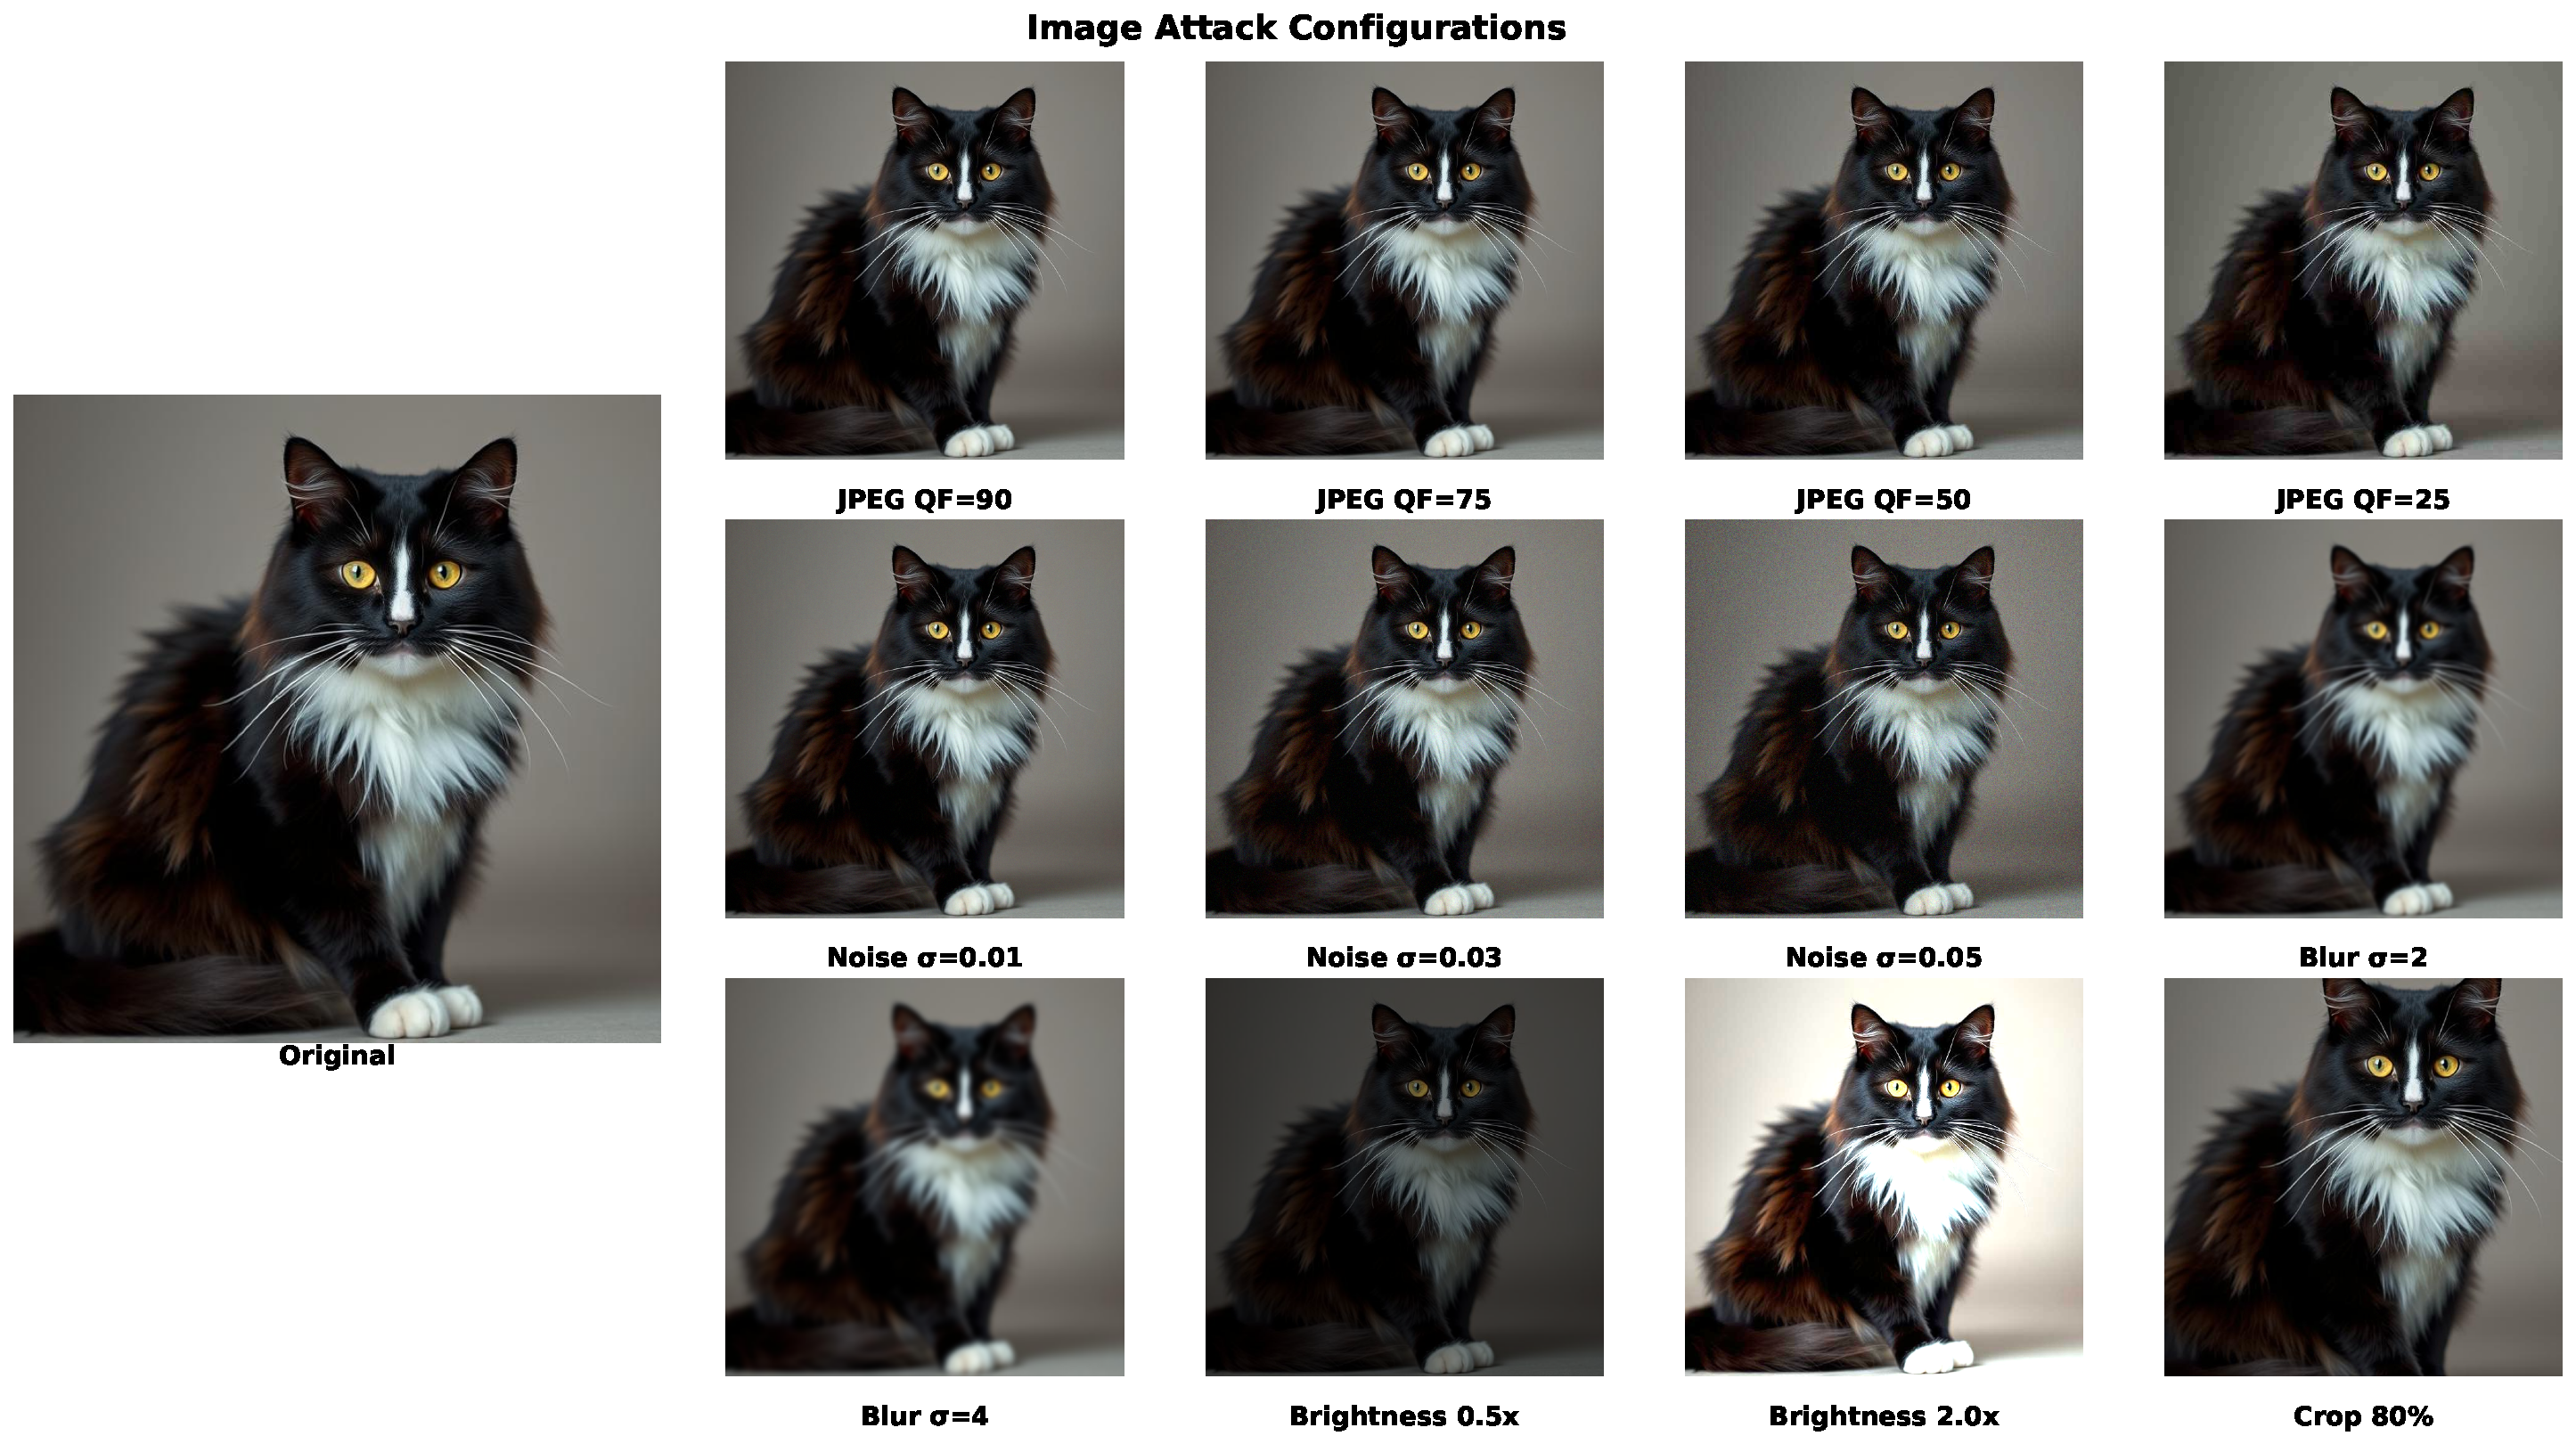
\includegraphics[width=\textwidth]{assets/image_attacks.pdf}
    \caption{A visual summary of the twelve digital attacks applied to evaluate watermark robustness.}
    \label{fig:image_attacks}
\end{figure}

\subsection{Evaluation Metrics}
\label{subsec:EvaluationMetrics}

The evaluation framework employs three metric categories.

While traditional metrics like \ac{PSNR} and \ac{SSIM} are common for assessing imperceptibility, they are not the primary metrics for this evaluation. The Gaussian Shading technique operates by altering the initial latent sample ($z_T$). As such, even when using an the same seed, the watermarked and non-watermarked images are inherently distinct at the pixel level, as they are slightly modified versions of one another. Applying pixel level metrics in this context is not appropriate, as they would report significant differences that do not reflect perceptual similarity.

Therefore, distribution based metrics are more appropriate. The \ac{FID} score is used to compare the statistical distributions of the entire set of 1000 watermarked images against the 1000 non-watermarked images, providing a more meaningful measure of the watermark's overall impact on the model's output distribution. Additionally, the \ac{CLIP} score is used to ensure that the semantic content of the generated images remains consistent with the original prompt, further validating the watermark's imperceptibility.

\textbf{Imperceptibility metrics} \ac{FID} for distribution preservation, and \ac{CLIP} Score for semantic similarity between prompts and generated images. \textbf{Robustness metrics} comprise \ac{BER} as the primary robustness measure, \ac{TPR} derived from accuracy measurements under the \ac{FPR}-controlled detection framework, and overall detection accuracy for binary classification performance. Statistical analysis will include $95\%$ confidence intervals for all key metrics and significance testing to assess performance differences across attack types.

\subsection{Comparative Analysis Strategy}
\label{subsec:ComparativeAnalysisStrategy}
A fundamental challenge in watermarking research is that differing papers will apply their own evaluation metrics and criteria, therefore making reliable comparisons difficult, without also implementing other methods using the same tests, which would be difficult for numerous reasons, for example, Stable Signature is not training agnostic, meaning deployment requires retraining of \ac{GAIM} training data. Acknowledging these limitations we shall compare methodological approaches rather than direct numerical benchmarking:

\begin{enumerate}
    \item \textbf{Methodological Analysis:} Focus on fundamental characteristics and trade-offs of different approaches (Tree-Ring \cite{wenTreeRingsWatermarksInvisible2023} and Stable Signature \cite{fernandezStableSignatureRooting2023b}).
    \item \textbf{Cross-Study Limitation Recognition:} Acknowledge that differences in experimental protocols, datasets, attack implementations, hardware configurations, and evaluation metrics can significantly influence reported performance figures.
    \item \textbf{Statistical Analysis:} Calculate $95\%$ confidence intervals for all key metrics using the 200 individual measurements per attack configuration. Perform statistical significance tests (paired t-tests, \ac{ANOVA}) to assess performance differences across attack types and intensities.
    \item \textbf{Independent Rigorous Evaluation:} Provide comprehensive statistical analysis of Gaussian Shading with $95\%$ confidence intervals and significance testing to enable future research to make informed comparisons.
\end{enumerate}

This approach prioritises methodological transparency and acknowledges the current limitations in \ac{AI} image watermarking.
\subsection{Statistical Rigour and Reproducibility}
\label{subsec:StatisticalRigor}

Scientific validity is ensured through deterministic random number generation with fixed seeds for reproducibility, statistically sufficient sample sizes (n=200 per attack, n=1000 for \ac{FID}), $95\%$ confidence intervals calculated using t-distribution, and comprehensive documentation of all code and hyperparameters under version control.

\subsection{Success Criteria and Thresholds}
\label{subsec:SuccessCriteria}

The evaluation sets a clear success criteria to assess Gaussian Shading's viability. \textbf{Imperceptibility thresholds} require \ac{FID} $<30$ (indicating minimal distribution shift between watermarked and non-watermarked images) and \ac{CLIP} Score difference $< 0.05$ (indicating preservation of semantic content). \textbf{Robustness thresholds} require \ac{BER} $< 0.1$ for mild attacks (\ac{JPEG} QF $\geq 75$), \ac{BER} $< 0.25$ for moderate attacks (\ac{JPEG} QF $\geq 50$), and \ac{TPR} $> 0.9$ at \ac{FPR} = $10^{-6}$. These derived thresholds from the literature provide objective criteria for evaluating the performance lossless claims of Gaussian Shading.

The methodology balances comprehensive evaluation with practical constraints, ensuring that results are both scientifically valid and directly comparable to existing literature while remaining achievable within undergraduate project scope and hardware limitations.


\chapter{Results and Analysis}
\label{cha:Results}

This chapter presents a comprehensive evaluation of the Gaussian Shading watermarking technique, examining its imperceptibility and robustness through  statistical analysis. The evaluation addresses the research questions concerning the viability of Gaussian Shading as a practical watermarking solution for \ac{AI}-generated images, and its place in the digital image watermarking landscape.

\section{Imperceptibility Analysis}
\label{sec:ImperceptibilityAnalysis}

The imperceptibility evaluation constitutes the foundational assessment of Gaussian Shading's main advantage: that watermarks can be embedded without degrading image quality. This analysis makes use of a varied approach, using semantic alignment metrics, and distributional statistics to provide a comprehensive understanding of the watermark's impact.

\subsection{Visual and Semantic Preservation}
\label{subsec:VisualSemanticPreservation}

Qualitative assessment confirms that the watermarking process consistently produces hig quality images. Figure \ref{fig:visual_comparison} demonstrates the framework's ability to generate visually appealing images across diverse categories, including landscapes, urban scenes, and food, with no additional artifacts or degradation. While a direct visual comparison of identical seeds is not feasible due to the nature of the sampling process, the consistent high quality across a wide range of content strongly suggests that the method preserves visual fidelity.

\begin{figure}[htb]
    \centering
    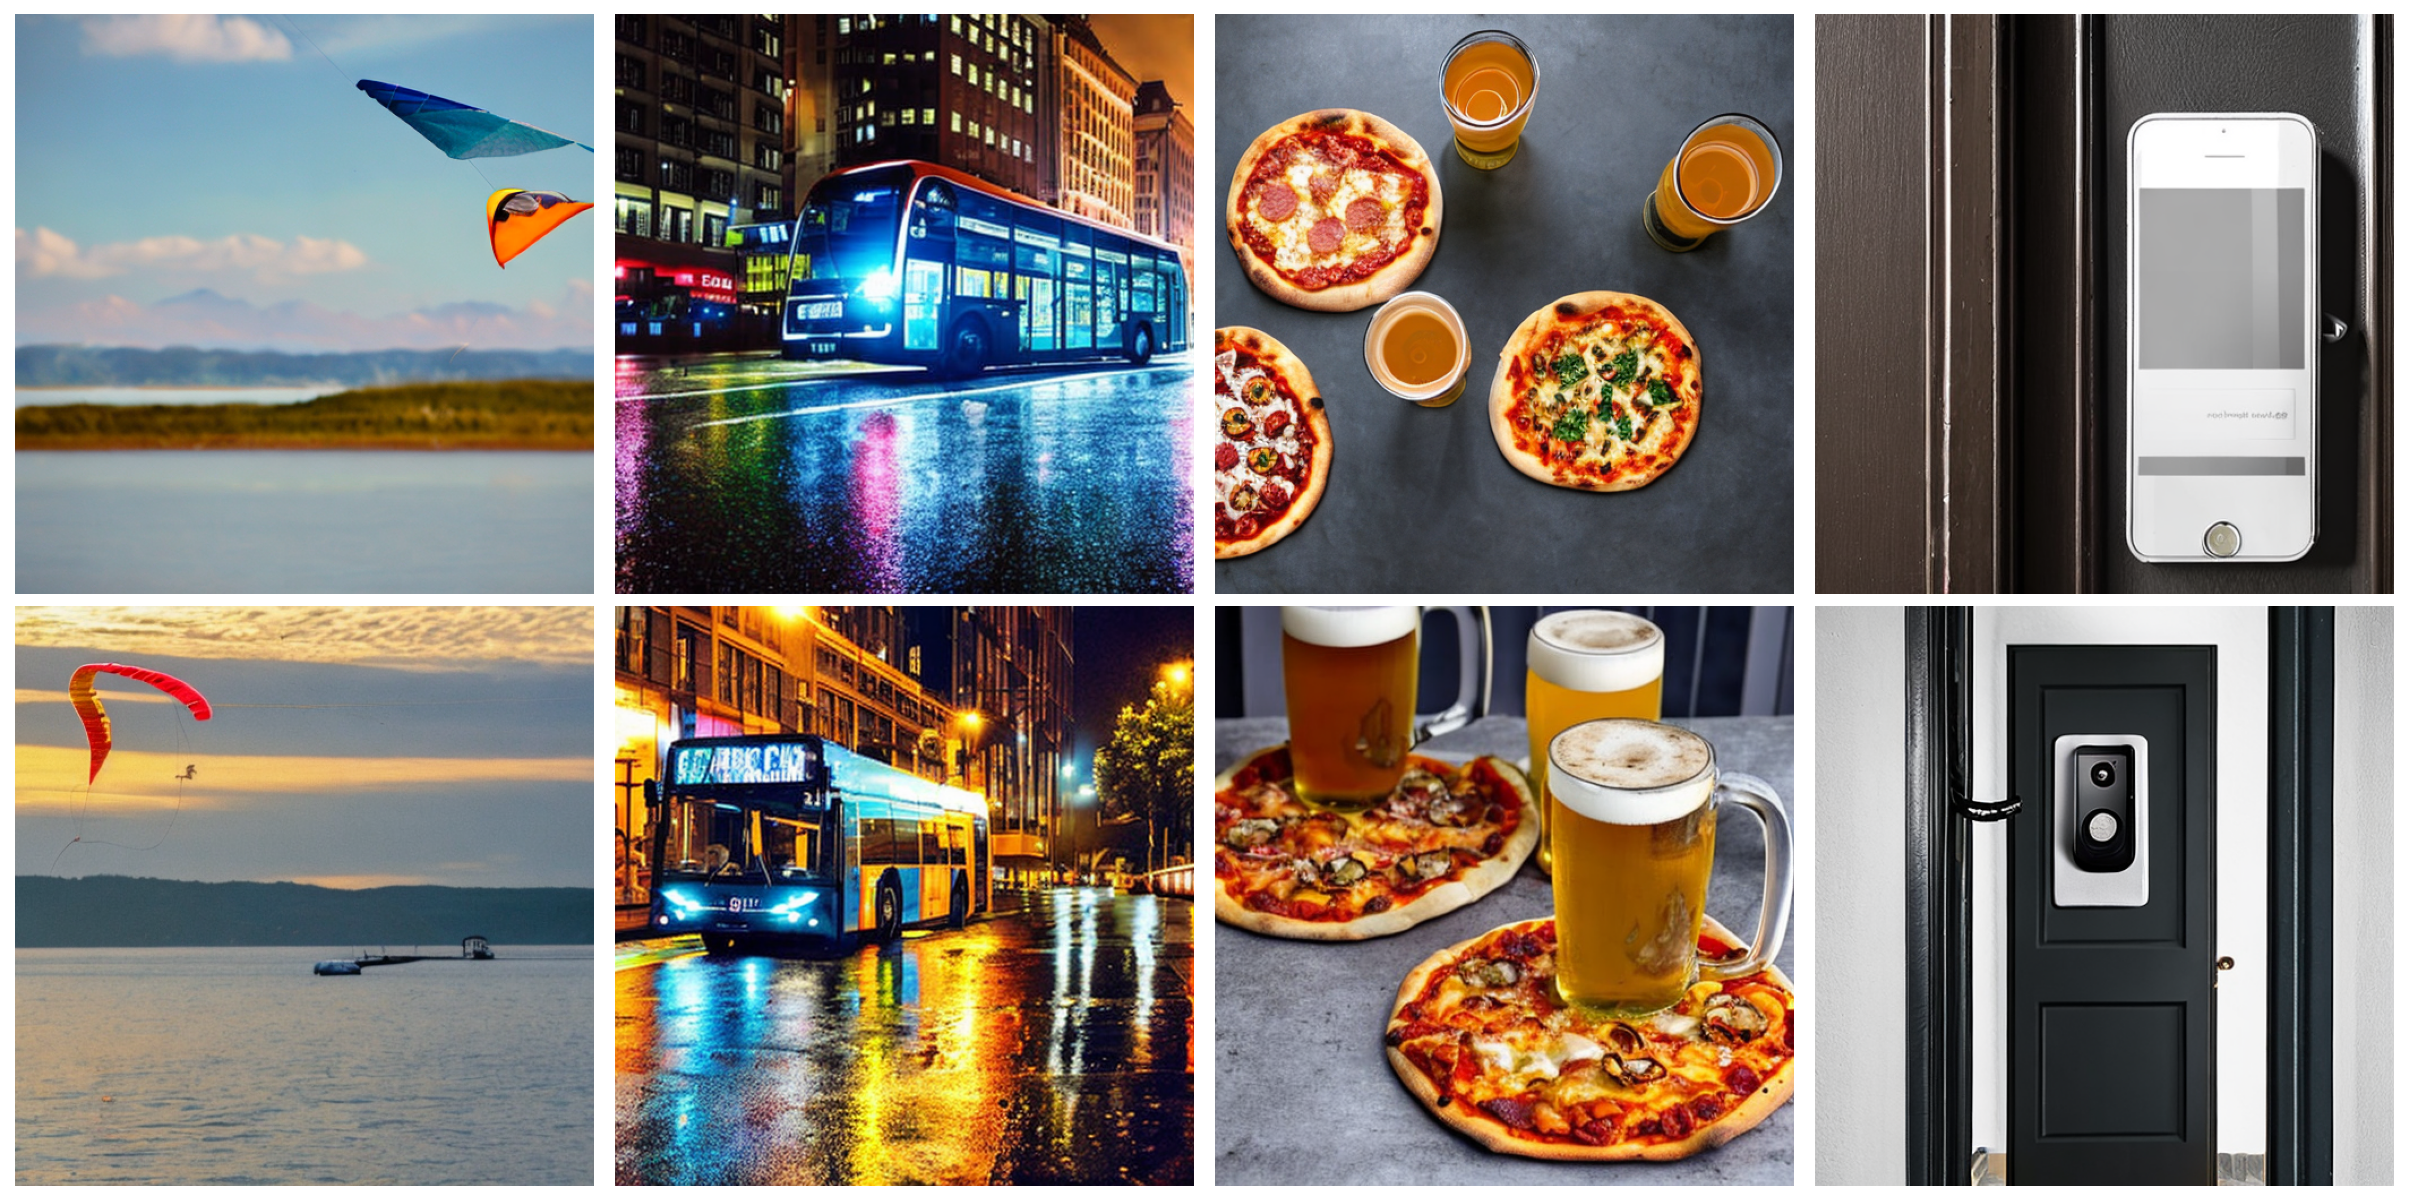
\includegraphics[width=\textwidth]{assets/visual_comparison.pdf}
    \caption{Sample images generated using the Gaussian Shading watermarking framework. The method maintains high visual quality across diverse content types, from landscapes and cityscapes to food and architectural subjects, with no discernible visual artifacts.}
    \label{fig:visual_comparison}
\end{figure}

To quantify semantic preservation, the evaluation uses \ac{CLIP} scores, which measure the semantic alignment between text prompts and the generated images. The results, presented in Table \ref{tab:semantic_metrics}, show remarkable semantic consistency. The negligible difference of $-0.0008$ between the watermarked $(0.3091)$ and non-watermarked $(0.3099)$ image sets is well within the bounds of natural variation and meets the success threshold of $< 0.05$. This confirms that the watermarking process does not interfere with the model's ability to generate images that remain faithful to their textual descriptions.

\begin{table}[htb]
    \caption{Semantic Preservation Analysis using CLIP Score}
    \label{tab:semantic_metrics}
    \begin{center}
    \begin{tabular}{|l|c|c|c|}
    \hline
    \textbf{Condition} & \textbf{Mean \ac{CLIP} Score} & \textbf{Difference} & \textbf{Assessment} \\ \hline
    Non-watermarked & $0.3099$ & - & Baseline \\ \hline
    Watermarked & $0.3091$ & $-0.0008$ & \textbf{Imperceptible} \\ \hline
    Success Threshold & - & $< 0.05$ & \textbf{Met} \\ \hline
    \end{tabular}
    \end{center}
\end{table}

The negligible difference in \ac{CLIP} scores (0.0008) demonstrates that the watermarking process preserves the semantic integrity of the generation process, ensuring that the resulting images remain faithful to their textual descriptions.

\subsection{Distributional Impact}
\label{subsec:DistributionalImpact}

While the visual and semantic assessments support the imperceptibility claims, the distributional analysis shows a different story. The \ac{FID} score, which measures the statistical distance between the distributions of the watermarked and non-watermarked image sets, yields a value of $47.83$. As shown in Table \ref{tab:distributional_metrics}, this is above the predefined success threshold of $30$, indicating a significant distributional shift between the 1000 watermarked and non-watermarked images.

This finding challenges the performance losslessness of Gaussian Shading. This high \ac{FID} score indicates that while individual images remain visually and semantically similar, the underlying statistical distribution of the watermarked image set has been measurably altered. This suggests that the watermarking process introduces systematic changes to the generative process that, while imperceptible at the individual image level, become detectable when analysing the aggregate behaviour of the model.

\begin{table}[htb]
    \caption{Distributional Metrics (FID Score)}
    \label{tab:distributional_metrics}
    \begin{center}
    \begin{tabular}{|l|c|c|c|}
    \hline
    \textbf{Metric} & \textbf{Observed Value} & \textbf{Success Threshold} & \textbf{Assessment} \\ \hline
    \ac{FID} Score & $47.83$ & $< 30$ & \textbf{Not Met} \\ \hline
    \end{tabular}
    \end{center}
\end{table}

\subsubsection{Understanding the FID Score}
The relatively high \ac{FID} score does not necessarily imply a degradation in the quality of individual images, but rather a shift in the overall distribution of the generated content. Several factors may contribute to this result:

\begin{enumerate}
    \item \textbf{Distributional Shift vs. Quality Degradation:} The high \ac{FID} score indicates a distributional shift rather than a drop in quality. The watermarking process modifies the initial latent sampling, which could alter the model's latent space in a way that affects overall statistics without compromising the quality of individual images.
    \item \textbf{Sample Size Sensitivity:} \ac{FID} scores are sensitive to sample size. This evaluation used 1000 images, whereas the original paper used 5000. This difference in scale may contribute to the elevated score through reduced statistical stability, although the core finding of a measurable impact remains valid.
    \item \textbf{Methodological Differences:} Minor variations in the \ac{FID} calculation methodology, such as the choice of feature extraction network or preprocessing steps, can also significantly impact results.
\end{enumerate}

\section{Statistical Analysis and Detection Performance}
\label{sec:StatisticalAnalysis}
This section provides comprehensive statistical analysis of the watermark detection performance, including \ac{FPR}/\ac{TPR} analysis under the algorithm's detection framework, confidence intervals for all key metrics, and statistical significance testing across attack types.

\subsection{FPR-Controlled Detection Framework}
\label{subsec:FPRControlledDetection}

The Gaussian Shading algorithm operates with an \ac{FPR}-controlled detection threshold, targeting an \ac{FPR} of $10^{-6}$ for statistical significance. Under this, the \ac{TPR} represents the algorithm's ability to correctly detect watermarked images at the controlled \ac{FPR}.

Table \ref{tab:fpr_tpr_analysis} presents the \ac{TPR} analysis derived from the accuracy measurements across all attack configurations, calculated from 200 samples per attack configuration using actual evaluation data. The results show excellent detection performance across all signal processing attacks, with \ac{TPR} values consistently above 98\%, except for failure under the geometric attack tested.

\begin{table}[htbp]
\centering
\caption{True Positive Rates with 95\% Confidence Intervals}
\label{tab:fpr_tpr_analysis}
\resizebox{\textwidth}{!}{%
\begin{tabular}{|l|c|c|c|c|}
\hline
\textbf{Attack Type} & \textbf{Parameter} & \textbf{TPR} & \textbf{95\% CI} & \textbf{n} \\
\hline
\multirow{2}{*}{brightness} & $0.500$ & $0.9994$ & $[0.9985, 1.0000]$ & $200$ \\
& $2.000$ & $0.9977$ & $[0.9950, 1.0000]$ & $200$ \\
\hline
crop & $0.800$ & $0.5148$ & $[0.5102, 0.5194]$ & $200$ \\
\hline
\multirow{2}{*}{gaussian\_blur} & $2.000$ & $0.9983$ & $[0.9962, 1.0000]$ & $200$ \\
& $4.000$ & $0.9820$ & $[0.9777, 0.9863]$ & $200$ \\
\hline
\multirow{3}{*}{gaussian\_noise} & $0.010$ & $0.9985$ & $[0.9961, 1.0000]$ & $200$ \\
& $0.030$ & $0.9963$ & $[0.9924, 1.0000]$ & $200$ \\
& $0.050$ & $0.9931$ & $[0.9890, 0.9972]$ & $200$ \\
\hline
\multirow{4}{*}{jpeg} & $25.000$ & $0.9865$ & $[0.9810, 0.9920]$ & $200$ \\
& $50.000$ & $0.9950$ & $[0.9905, 0.9995]$ & $200$ \\
& $75.000$ & $0.9972$ & $[0.9938, 1.0000]$ & $200$ \\
& $90.000$ & $0.9983$ & $[0.9956, 1.0000]$ & $200$ \\
\hline
\end{tabular}%
}
\end{table}

The analysis shows exceptional \ac{TPR} performance across all signal processing attacks, with values consistently above $98\%$ even under severe conditions. However, the geometric attack (crop) results in \ac{TPR} failure at $51.48\%$, statistically indistinguishable from random chance.

\subsection{Statistical Significance}
\label{subsec:StatisticalSignificance}

To assess the statistical significance of performance differences across attack types and intensities, one-way \ac{ANOVA} and paired t-tests were conducted on the \ac{BER} measurements from the 200 generated images per attack configuration.

\subsubsection{Attack Type Comparison}
One-way \ac{ANOVA} testing across the five main attack categories (brightness, Gaussian blur, Gaussian noise, jpeg, crop) shows significant differences in robustness performance ($F(4,2395) = 15064.930$, $p < 0.001$). Post-hoc Tukey \ac{HSD} tests identify that:

\begin{itemize}
    \item \textbf{Crop attacks} show much worse performance compared to all other categories ($p < 0.001$)
    \item \textbf{Brightness attacks} show significantly superior robustness compared to all other categories ($p < 0.001$)
    \item \textbf{Gaussian blur} shows worse performance than brightness, JPEG, and noise attacks ($p < 0.001$)
    \item \textbf{JPEG compression} and \textbf{Gaussian noise} show comparable performance ($p = 0.740$, not significant)
\end{itemize}

\subsubsection{Attack Intensity Analysis}
Paired t-tests examining performance degradation with increasing attack intensity show statistically significant effects:

\begin{itemize}
    \item \textbf{Brightness intensity:} Factor $0.5$ vs $2.0$ ($t = 1.876$, $p = 0.062$, marginally significant)
    \item \textbf{Gaussian blur intensity:} Radius $2.0$ vs $4.0$ ($t = 11.121$, $p < 0.001$, highly significant)
    \item \textbf{Gaussian noise intensity:} Progressive degradation across $\sigma$ levels ($0.01$ vs $0.03$: $t = 2.498$, $p = 0.013$; $0.03$ vs $0.05$: $t = 4.699$, $p < 0.001$)
    \item \textbf{JPEG compression intensity:} Significant degradation with decreasing quality (QF $25$ vs $50$: $t = -6.157$, $p < 0.001$; QF $50$ vs $75$: $t = -3.150$, $p = 0.002$; QF $75$ vs $90$: $t = -2.533$, $p = 0.012$)
\end{itemize}

These results provide statistical validation that the observed performance patterns are not due to random variation but represent genuine algorithmic characteristics, with the crop attack showing the most dramatic performance degradation.

This analysis suggests that while Gaussian Shading achieves excellent visual and semantic imperceptibility, it is not entirely performance lossless from a distributional perspective. This has implications for applications where maintaining precise distributional properties is critical, and highlights the need for a multi faceted understanding of imperceptibility in watermarking research.

\section{Robustness Evaluation}
\label{sec:RobustnessEvaluation}

The robustness assessment evaluates the watermark's resilience against a comprehensive suite of attacks designed to simulate real world image manipulations. This analysis reveals the methods exceptional strength against signal processing attacks but vulnerability to geometric transformations. This section discusses these results, providing a detailed analysis of the method's strengths and its limitations.

\subsection{Robustness to Signal Processing Attacks}
\label{subsec:SignalProcessingRobustness}

The evaluation of signal processing attacks shows Gaussian Shading's remarkable robustness against common image degradations. Figure \ref{fig:robustness_jpeg_noise} illustrates the watermark's resilience to two of the most critical attack categories: \ac{JPEG} compression and additive Gaussian noise.

\begin{figure}[htb]
    \centering
    \includegraphics[width=\textwidth]{assets/robustness_jpeg_noise.pdf}
    \caption{Robustness against signal processing attacks. Left: \ac{JPEG} compression robustness, showing minimal degradation, despite aggressive compression ratios. Right: Gaussian noise resilience, demonstrating consistent performance across increasing noise levels.}
    \label{fig:robustness_jpeg_noise}
\end{figure}

\subsubsection{JPEG Compression and Noise Resilience}
The \ac{JPEG} compression results are particularly impressive. Even under severe compression (quality factor $25$), the \ac{BER} remains at $0.0135\ (1.35\%)$, far below the established success threshold of $0.25$ for moderate attacks. This performance is noteworthy, as \ac{JPEG} compression is one of the most common and destructive operations for many watermarking schemes. Similarly, the watermark maintains excellent detectability under significant Gaussian noise ($\sigma = 0.05$), with the \ac{BER} reaching only $0.0069\ (0.69\%)$.

This high level of robustness can be attributed to the method's operation in the latent space. By embedding the watermark in the initial latent vector and preserving its statistical properties, Gaussian Shading creates a watermark that is deeply integrated with the image's fundamental structure, making it resilient to attacks that primarily affect the pixel level or high frequency information.

\subsubsection{Additional Signal Processing Attacks}
The method's strong performance extends to other signal processing attacks. As detailed in Table \ref{tab:comprehensive_robustness}, Gaussian blur with a radius of $4$ pixels results in a \ac{BER} of only $0.0180\ (1.8\%)$, while brightness adjustments across a factor-of-four range $(0.5\times$ to $2.0\times)$ yield a negligible maximum \ac{BER} of $0.0023\ (0.23\%)$. This combination of results establish Gaussian Shading as exceptionally robust against a broad range of signal processing attacks, positioning it favourably against the many other existing modern \ac{AI} image watermarking techniques.

\subsection{Vulnerability to Geometric Attacks}
\label{subsec:GeometricVulnerability}

In stark contrast to its signal processing robustness, the evaluation reveals a vulnerability to geometric attacks. Figure \ref{fig:robustness_blur_crop} illustrates this, showing the failure under a random crop attack compared to the impressive resilience against a strong blur.

\begin{figure}[htb]
    \centering
    \includegraphics[width=\textwidth]{assets/robustness_blur_crop.pdf}
    \caption{Left: Continued excellent performance against Gaussian blur. Right: The failure under a crop attack (red bar) compared to the maintained robustness against other severe signal processing attacks.}
    \label{fig:robustness_blur_crop}
\end{figure}

The crop attack, which removes $20\%$ of the image area before resizing, results in a high \ac{BER} of $ 0.4852\ (48.52\%)$. A value statistically indistinguishable from random guessing $(50\%)$. This represents a complete failure of the watermark, indicating that the method's spatial redundancy is insufficient to survive significant data loss.

\subsubsection{Root Cause Analysis of Geometric Failure}
The failure for cropping is due to the fundamental limitations of the Gaussian Shading algorithm:
\begin{enumerate}
    \item \textbf{Lack of Geometric Invariance:} The method lacks inherent geometric invariance. The watermark's structure is tied to the absolute spatial coordinates of the latent space, therefore any transformation that changes these relationships (like cropping or rotation) desynchronises the extraction process.
    \item \textbf{Insufficient Spatial Redundancy:} While the watermark is diffused across spatial dimensions, the level of redundancy is not sufficient to reconstruct the message when a significant, contiguous section of the image is removed.
    \item \textbf{No Integrated Error Correction:} The base algorithm does not make use of sophisticated error correction codes (such as Reed-Solomon \cite{reedPolynomialCodesCertain1960}) that are specifically designed to handle errors caused by spatial data loss.
\end{enumerate}
This vulnerability has practical implications, as cropping is a common image manipulation, from images being shared online such as in social media posts and academic publications.

\subsection{Comparative Performance and Overall Assessment}
\label{subsec:RobustnessOverview}

Table \ref{tab:comprehensive_robustness} provides a complete overview of the robustness evaluations conducted, clearly showing the method's strengths and limitations. These results show great robustness against signal processing attacks along with a failure against geometric transformations (crop).

\begin{table}[htb]
    \caption{Comprehensive Robustness Evaluation Results with Statistical Confidence}
    \label{tab:comprehensive_robustness}
    \begin{center}
    \resizebox{\textwidth}{!}{%
    \begin{tabular}{|l|l|c|c|c|c|}
    \hline
    \textbf{Attack Category} & \textbf{Attack Configuration} & \textbf{Mean \ac{BER}} & \textbf{95\% CI} & \textbf{Performance} & \textbf{Assessment} \\ \hline
    \multirow{4}{*}{JPEG Compression} & Quality=$90$ & $0.0017$ & $\pm 0.0027$ & Excellent & \textbf{Pass} \\
     & Quality=$75$ & $0.0028$ & $\pm 0.0034$ & Excellent & \textbf{Pass} \\
     & Quality=$50$ & $0.0050$ & $\pm 0.0045$ & Excellent & \textbf{Pass} \\
     & Quality=$25$ & $0.0135$ & $\pm 0.0055$ & Very Good & \textbf{Pass} \\ \hline
    \multirow{3}{*}{Gaussian Noise} & $\sigma=0.01$ & $0.0015$ & $\pm 0.0024$ & Excellent & \textbf{Pass} \\
     & $\sigma=0.03$ & $0.0037$ & $\pm 0.0040$ & Excellent & \textbf{Pass} \\
     & $\sigma=0.05$ & $0.0069$ & $\pm 0.0041$ & Excellent & \textbf{Pass} \\ \hline
    \multirow{2}{*}{Gaussian Blur} & Radius=$2$ & $0.0017$ & $\pm 0.0020$ & Excellent & \textbf{Pass} \\
     & Radius=$4$ & $0.0180$ & $\pm 0.0043$ & Very Good & \textbf{Pass} \\ \hline
    \multirow{2}{*}{Brightness} & Factor=$0.5$ & $0.0006$ & $\pm 0.0009$ & Excellent & \textbf{Pass} \\
     & Factor=$2.0$ & $0.0023$ & $\pm 0.0027$ & Excellent & \textbf{Pass} \\ \hline
    \textbf{Geometric} & \textbf{Crop (80\% retention)} & \textbf{0.4852} & $\pm 0.0046$ & \textbf{Very Poor} & \textbf{Fail} \\ \hline
    \end{tabular}%
    }
    \end{center}
    \footnotesize{\textit{Confidence intervals calculated using t-distribution for n=200 samples per attack configuration.}}
\end{table}

To contextualise these findings, Table \ref{tab:comparative_robustness} presents a methodological comparison with Tree-Ring \cite{wenTreeRingsWatermarksInvisible2023} and Stable Signature \cite{fernandezStableSignatureRooting2023b}.

The comparison reveals distinct positioning within the watermarking landscape. Gaussian Shading shares with Tree-Ring the advantage of training-free deployment, enabling rapid integration into existing systems without requiring model retraining. However, it substantially exceeds its capacity limitations (256 bits vs. 1 bit), making it more suitable for detailed attribution and traceability applications. Compared to Stable Signature, Gaussian Shading's plug-and-play deployment represents a practical advantage, though this simplicity may come at the cost of the geometric robustness that fine-tuned approaches can achieve.

This methodological analysis highlights a key challenge in watermarking research: the difficulty of making reliable cross-study performance comparisons due to variations in experimental protocols, datasets, attack implementations, and evaluation metrics. Such differences can significantly influence reported performance figures, for direct numerical comparisons an identical evaluation framework should be used.

\begin{table}[htb]
    \caption{Comparison of Watermarking Techniques}
    \label{tab:comparative_robustness}
    \begin{center}
    \resizebox{\textwidth}{!}{%
    \begin{tabular}{|l|c|c|c|}
    \hline
    \textbf{Characteristic} & \textbf{Gaussian Shading (This work)} & \textbf{Tree-Ring \cite{wenTreeRingsWatermarksInvisible2023}} & \textbf{Stable Signature \cite{fernandezStableSignatureRooting2023b}} \\
    \hline
    \textbf{Embedding Domain} & Latent (Initial Sampling) & Latent (Initial Noise) & Model (\ac{VAE} Fine-tuning) \\
    \hline
    \textbf{Training Required} & None & None & Yes (\ac{VAE} fine-tuning) \\
    \hline
    \textbf{Watermark Capacity} & 256 bits & 1 bit & 64 bits \\
    \hline
    \textbf{Integration Approach} & Distribution-preserving sampling & \ac{DDIM} noise injection & Decoder modification \\
    \hline
    \textbf{Signal Processing Robustness} & High (\ac{BER} < 2\%) & Reported as high & Reported as high \\
    \hline
    \textbf{Geometric Attack Robustness} & Poor (Crop: \ac{BER} 48.5\%) & Reported as moderate & Reported as good \\
    \hline
    \textbf{Deployment Complexity} & Low (plug-and-play) & Low (plug-and-play) & High (requires retraining) \\
    \hline
    \textbf{Model Architecture} & Any \ac{LDM} & Diffusion Models & Stable Diffusion specific \\
    \hline
    \end{tabular}%
    }
    \end{center}
\end{table}

This comparative analysis solidifies the conclusion that Gaussian Shading occupies a specific niche: it is a high-capacity, easy-to-deploy solution that offers excellent protection in environments where geometric transformations are unlikely. However, its critical failure under cropping makes it unsuitable for applications where such manipulations are common.

\section{Evaluation Scale and Statistical Methodology}
\label{sec:EvaluationScale}

The robustness evaluation was based on 200 images per attack configuration totalling 2400 individual experiments, providing a substantial dataset for statistical analysis. The imperceptibility assessment was conducted on 1000 image pairs for the \ac{FID} calculation and \ac{CLIP} score comparison.

The comprehensive nature of the evaluation, spanning multiple attack types and intensities, enables reliable conclusions about the method's performance across differing scenarios. The sample sizes ($n=200$ per attack) provide adequate data for calculating meaningful $95\%$ confidence intervals using t-distribution and conducting significance testing through \ac{ANOVA} and paired t-tests. This analysis ensures that the observed performance patterns are representative and statistically validated rather than artifacts of limited testing or random variation.

\section{Comparative Contextualisation}
\label{sec:ComparativeContext}

When positioned within the broader landscape of \ac{AI} watermarking techniques, Gaussian Shading's performance profile reveals both distinctive advantages and notable limitations. Compared to Stable Signature's requirement for model fine-tuning, Gaussian Shading's training-free nature represents a significant practical advantage, enabling rapid deployment across existing infrastructure without retraining costs.

Against Tree-Ring's 1-bit capacity limitation, Gaussian Shading's 256-bit payload capability provides substantial advantages for attribution and traceability applications. However, this capacity comes at the cost of the geometric vulnerability identified in this evaluation.

The distributional impact revealed through \ac{FID} analysis positions Gaussian Shading between truly lossless methods and those with more pronounced quality degradation. This intermediate position reflects the fundamental trade-offs inherent in watermarking system design.

\section{Key Research Questions: Empirical Answers}
\label{sec:ResearchAnswers}

The evaluation provides definitive empirical answers to the study's fundamental research questions:

\textbf{Research Question 1: Robustness Extent}
Gaussian Shading demonstrates exceptional robustness against signal processing attacks, with \ac{BER} consistently below $2\%$ even under severe conditions. However, it exhibits vulnerability to geometric attacks, particularly cropping, where performance degrades to random-chance levels.

\textbf{Research Question 2: Performance/Quality Trade-offs}
The method achieves visual and semantic imperceptibility, confirming its claims at the perceptual level. However, distributional analysis reveals measurable impact on the generative model's statistical properties, challenging absolute "performance-lossless" claims.

\textbf{Research Question 3: Competitive Positioning}
Gaussian Shading offers unique advantages in training-free deployment and high capacity, but these benefits come with the trade-off of geometric vulnerability and measurable distributional impact. The method occupies a distinct niche in the watermarking landscape, optimised for specific use cases rather than universal application.

\chapter{Conclusion}
\label{cha:conclusion}

This dissertation has conducted a comprehensive, independent evaluation of the Gaussian Shading watermarking technique across 2400 individual robustness experiments, providing insights into its performance and practical viability. Through implementation and systematic evaluation with statistical validation. The evaluation revealed exceptional robustness against signal processing attacks, with \ac{TPR} values consistently above $98\%$ across all tested conditions, while statistical analysis using one-way \ac{ANOVA} confirmed performance differences across attack categories ($F(4,2395) = 15064.930$, $p < 0.001$). The findings challenge the absoluteness of Gaussian Shadings performance losslessness by revealing a measurable distributional impact despite perceptual imperceptibility. Furthermore, the research provides a definitive analysis of the method's robustness, highlighting the resilience to most common signal processing attacks but a vulnerability to geometric transformations, with the cropping attack resulting in performance statistically indistinguishable from random chance (\ac{TPR} $51.48\%$, $95\%$ confidence interval $[51.02\%, 51.94\%]$).

This work presents a nuanced understanding of the trade-offs inherent in the Gaussian Shading watermarking method through statistical analysis with $95\%$ confidence intervals derived from 200 samples per attack configuration. By providing detailed performance data with statistical validation, this project serves as a starting point for future research with actionable insights, particularly the need to further evaluate and enhance geometric robustness. The statistical methods employed reveal brightness attacks as the least destructive to watermark retrieval. Ultimately, this dissertation highlights the importance of an in depth evaluation with statistical validation and contributes to the development of more reliable and effective solutions for ensuring the authenticity and traceability of \ac{AI}-generated images.

\section{Limitations}
\label{sec:LimitationsAlternatives}

While this evaluation provides significant insights, there are several limitations to consider. The evaluation is limited to a single model architecture (Stable Diffusion v2.1), and its findings may not directly transfer to other \acp{LDM} or generative models. The attack suite, while comprehensive, did not include sophisticated adversarial attacks designed to specifically target the watermarking algorithm, which could reveal further vulnerabilities. Additionally, hardware constraints necessitated a smaller dataset for \ac{FID} calculation (1000 images) than the original paper (5000 images), which may contribute to the elevated score. Furthermore, only a single geometric attack (random cropping) was evaluated, which limits the understanding of the method's robustness against other geometric transformations such as rotation or scaling. This is especially relevant given the method's vulnerability to cropping, which is a common image manipulation in real-world scenarios.

\section{Future Work and Implications}
\label{sec:FutureWorkImplications}

The findings from this research open several promising avenues for future investigation and have significant implications for the responsible development of \ac{AI}.

\subsection{Future Research Directions}
The most critical area for future work is more research into geometric robustness. This could be achieved by integrating advanced error correction codes (e.g., \ac{BCH} Reed-Solomon \cite{reedPolynomialCodesCertain1960}), developing spatial redundancy schemes, or exploring geometric invariant feature spaces for embedding. Another key point is mitigating the distributional impact identified by the relatively high \ac{FID} score. This would involve analysis at a larger scale (e.g. larger datasets). Finally, future work should focus on use of a standardised benchmarking framework such as WAVES \cite{anWAVESBenchmarkingRobustness2024} by applying the same evaluation techniques across a diverse range of generative architectures and assessing resistance against sophisticated adversarial attacks.

\subsection{Implications for Responsible AI}
This research provides insights for the broader development of responsible \ac{AI} systems. For policy and regulation, the findings demonstrate that while watermarking is a promising tool, its limitations (e.g. geometric vulnerability) must be considered when deploying a suitable method for widespread use. This work highlights the need for more nuanced, multi faceted evaluation frameworks and pinpoints geometric robustness as a key area for future research. By contributing an independent assessment, this study helps build a foundation for developing more reliable and effective technologies for digital content authentication in the age of \ac{AI}.

\appendix
\chapter{Appendix}
\label{app:AdditionalContent}

\section{Gaussian Shading sampling function}
\begin{lstlisting}[language=Python, caption={Gaussian Shading Sampling Implementation}]
def distribution_preserving_sampling(z_t, m, alpha=0.5):
    # Convert to uniform using normal CDF
    u_z = 0.5 * (1 + torch.erf(z_t / math.sqrt(2)))
    
    # Create reference latent based on watermark bit
    z_ref = torch.randn_like(z_t)
    u_ref = 0.5 * (1 + torch.erf(z_ref / math.sqrt(2)))
    
    # Adjust reference values based on watermark bits
    mask = (m > 0.5).float()
    u_ref = mask * torch.clamp(u_ref, min=0.5) + (1 - mask) * torch.clamp(u_ref, max=0.5)
    
    # Interpolate in uniform space
    u_mix = alpha * u_z + (1 - alpha) * u_ref
    
    # Convert back to normal distribution
    # Clamp to avoid numerical issues at extremes
    u_mix_safe = torch.clamp(u_mix, min=1e-6, max=1-1e-6)
    z_watermarked = math.sqrt(2) * torch.erfinv(2 * u_mix_safe - 1)
    
    return z_watermarked
\end{lstlisting}

\section{Watermark Evaluation Logic}
This function implements the main part of watermark detection, supporting the \ac{BER} calculations in the results.
\begin{lstlisting}[language=Python, caption={Watermark Detection and Evaluation Implementation}]
def eval_watermark(self, reversed_m):
    # Convert latent values to binary (threshold at 0)
    reversed_m = (reversed_m > 0).int()
    
    # Decrypt the watermark using the stored key
    reversed_sd = (reversed_m + self.key) % 2
    
    # Apply diffusion inverse to reconstruct watermark
    reversed_watermark = self.diffusion_inverse(reversed_sd)
    
    # Calculate accuracy by comparing with original watermark
    correct = (reversed_watermark == self.watermark).float().mean().item()
    
    # Update detection counters based on thresholds
    if correct >= self.tau_onebit:
        self.tp_onebit_count = self.tp_onebit_count + 1
    if correct >= self.tau_bits:
        self.tp_bits_count = self.tp_bits_count + 1
    
    return correct
\end{lstlisting}

\section{GPU Memory Optimisation}
This function enabled large scale evaluation (2400 robustness experiments, 1000 imperceptibility experiments) on consumer hardware (RTX 2070 Super, 8GB VRAM).
\begin{lstlisting}[language=Python, caption={GPU Memory Optimisation}]
def optimise_gpu_memory():
    """Optimise GPU memory usage."""
    if torch.cuda.is_available():
        torch.cuda.empty_cache()
        torch.cuda.synchronize()
        # Enable memory efficient attention if available
        try:
            torch.backends.cuda.enable_flash_sdp(True)
        except:
            pass
\end{lstlisting}

\section{Statistical Analysis Code Snippets}
This section provides key Python code snippets from the statistical analysis script for reproducibility.
% \subsection{Confidence Interval Calculation}
\begin{lstlisting}[language=Python, caption={Confidence Interval Calculation}]
import scipy.stats as stats
import numpy as np

def calculate_confidence_intervals(data, confidence=0.95):
    n = len(data)
    mean = np.mean(data)
    std_err = stats.sem(data)
    t_critical = stats.t.ppf((1 + confidence) / 2, n - 1)
    margin = t_critical * std_err
    
    lower_bound = max(0, mean - margin)
    upper_bound = min(1, mean + margin)
    
    return mean, lower_bound, upper_bound, margin, t_critical
\end{lstlisting}

% \subsection{ANOVA Analysis}
\begin{lstlisting}[language=Python, caption={ANOVA Analysis}]
from scipy.stats import f_oneway
from statsmodels.stats.multicomp import pairwise_tukeyhsd

# Group data by attack type
attack_groups = []
attack_types = ['brightness', 'crop', 'gaussian_blur',
                'gaussian_noise', 'jpeg']
for attack_type in attack_types:
    attack_data = detailed_data[
        detailed_data['attack_name'] == attack_type
    ]['ber'].values
    attack_groups.append(attack_data)

# Perform one-way ANOVA
f_stat, p_value = f_oneway(*attack_groups)

# Tukey HSD post-hoc test
tukey_results = pairwise_tukeyhsd(
    endog=detailed_data['ber'],
    groups=detailed_data['attack_name'],
    alpha=0.05
)
\end{lstlisting}

\chapter{Ethics Checklist}
\label{app:EthicsChecklist}
\section*{Ethical Considerations Checklist and Declaration}

\subsection*{Project Description}
\textit{Briefly explain the methodology of your study. Give sufficient detail that a non-expert in the subject can understand what you are proposing to do.}

\vspace{1em}
\noindent
\begin{tabularx}{\textwidth}{|X|}
\hline
Identifying images generated by Artificial Intelligence (AI) with invisible watermarks: This can help improve copyright protections, traceability, and accountability. A watermarking method will be implemented to embed and retrieve these imperceptible watermarks with minimal compromise to quality. The method will be evaluated against its resistance to common attacks such as compression, cropping, noise, and smoothing. Additionally the chosen method will be compared with existing methods. \\
\hline
\end{tabularx}

\subsection*{External Datasets}
\textit{If you are using external datasets, please (a) identify the dataset(s) giving sufficient details; (b) identify the relevant licence or terms of use for the dataset(s) and justify why your project would be compliant with those terms; (c) if the data is about humans, also provide evidence that the data was initially collected with consent.}

\vspace{1em}
\noindent
\begin{tabularx}{\textwidth}{|X|}
\hline
The project will make use of text-to-image prompt datasets in order to have standardisation of generated images COCO-2017 (CC BY-SA 4.0), Meaning attribution is required. The project will be compliant with the terms as no changes are being made and the datasets used will be credited and referenced Gustavosta prompt set. \\
\hline
\end{tabularx}

\subsection*{Potential Ethical Issues}
\textit{Does your project involve any of the following? Please mark Yes or No for \textbf{all} issues.}

\vspace{1em}
\noindent
\begin{tabularx}{\textwidth}{|X|c|}
\hline
\textbf{Issue} & \textbf{Yes / No} \\
\hline
Human participants (adults or children) & No \\
\hline
Human data (e.g. data collected through surveys and questionnaires on issues such as lifestyle, housing and working environments, or attitudes and preferences, or datasets including human data) & No \\
\hline
Datasets that require permission from the data provider & No \\
\hline
Applications that could potentially involve unethical practice, including potential dual-use applications (e.g. projects involving tools or data that can be used for unethical purposes e.g. to attack systems) & No \\
\hline
Funding sources or collaboration with potential to adversely affect existing relationships or bring the University or Department into disrepute (e.g. projects related to gambling, dark market, etc.) & No \\
\hline
Restrictions on dissemination (e.g. not being allowed to publish certain datasets or results) & No \\
\hline
Military or defence context & No \\
\hline
Overseas countries under regimes with poor human rights record or identified as dangerous by the Foreign \& Commonwealth Office & No \\
\hline
Human material (e.g. tissue or fluid samples), vertebrates, especially mammals and birds, or any other organisms not previously mentioned & No \\
\hline
\end{tabularx}

\vspace{1em}
\noindent
\textit{If you answered \textbf{No} to all the above, you do not need ethical approval.}

\vspace{1em}
\noindent
\textit{If you answered \textbf{Yes} to any of the above, you must complete a Fast-Track Ethical Approval Form, get it signed off by your project advisor, and submit it for approval to the Departmental Ethics Officers.}

\subsection*{Student Declaration}
\textit{I have considered the ethical implications of this project, all the terms and conditions and permissions of any datasets being used, and I have identified no significant ethical implications requiring an ethical approval application.}

\vspace{1em}
\noindent
\begin{tabularx}{\textwidth}{|l|X|}
\hline
\textbf{Student Name} & Mischa Zaynchkovsky \\
\hline
\textbf{Student Signature} & Mischa Zaynchkovsky \\
\hline
\textbf{Date} & 14/02/2025 \\
\hline
\end{tabularx}

\sloppy % relax spacing between words
\printbibliography

\end{document}
